\documentclass[11pt]{article}
\usepackage[a4paper,top=25mm,bottom=25mm,left=24mm,right=24mm]{geometry}
\usepackage{fontspec}
\usepackage{amsmath,amssymb,amsthm,mathtools}
\usepackage{booktabs,array,tabularx}
\usepackage{enumitem}
\usepackage{caption}
\usepackage[hidelinks,unicode]{hyperref}
\usepackage{bookmark}
\usepackage{setspace}
\usepackage{graphicx}

% --- fonts (XeLaTeX, no xeCJK available; use fontspec + ICU line breaking) ---
\setmainfont{Noto Serif CJK JP}
\newfontfamily\jpg{Noto Sans CJK JP}
\XeTeXlinebreaklocale "ja"
\XeTeXlinebreakskip=0pt plus 0.1pt minus 0.01pt
\linespread{1.18}

% --- math display spacing ---
\setlength{\jot}{4pt}
\allowdisplaybreaks

% --- theorem environments ---
\theoremstyle{plain}
\newtheorem{prop}{命題}
\newtheorem{cor}{系}
\theoremstyle{definition}
\newtheorem{defn}{定義}
\newtheorem{assm}{仮定}
\theoremstyle{remark}
\newtheorem*{rmk}{注}

% --- section heading look ---
\usepackage{titlesec}
\titleformat{\section}{\large\bfseries\sffamily}{\thesection}{0.6em}{}
\titleformat{\subsection}{\normalsize\bfseries\sffamily}{\thesubsection}{0.6em}{}
\titleformat{\subsubsection}{\normalsize\bfseries\sffamily}{\thesubsubsection}{0.6em}{}
\renewcommand{\sffamily}{\jpg}

% --- boxed-claim helper ---
\usepackage[most]{tcolorbox}
\newtcolorbox{claimbox}[1][]{colback=black!3,colframe=black!55,boxrule=0.4pt,
  arc=1.2pt,left=6pt,right=6pt,top=5pt,bottom=5pt,#1}

\captionsetup{font=small,labelfont=bf,labelsep=quad}
\setlength{\parindent}{1em}

\title{\bfseries 知能の民主化と労働市場再編\\[2pt]
\large 監督ボトルネックが成立する条件\\[2pt]
\normalsize ── 有限の監督供給の下でAI普及が労働負荷へ転嫁される制度条件 ──}
%% TODO-AUTHOR: 著者名・所属を記入してから投稿・公開すること
\author{\normalsize ［著者名・所属を記入］}
\date{\normalsize 研究論文ドラフト 第12版（理論＋タスク側パラメータの較正）\\ 2026年7月（v12）・公開AI利用データによる較正と測定監査を追加}

\begin{document}
\maketitle
\thispagestyle{empty}

\begin{center}
\small\itshape 未定稿（Working Paper）。引用・配布の際はその旨を明記されたい。コメントを歓迎する。
\end{center}
\vspace{2mm}
\section*{要旨}
\small
AI利用と労働時間の関係について、既存の実証研究は割れている。米国の生活時間日誌を用いた研究はAI曝露が高い職業ほど労働時間が長いと報告し（Jiang et al., 2025）、デンマークの行政記録を用いた研究は賃金・労働時間のいずれにも精密なゼロを報告する（Humlum and Vestergaard, 2025）。本稿は、この対立が\emph{制度条件の違い}として整合的に説明できることを示す。すなわち、AI普及が専門職の労働負荷へ転嫁される\emph{条件}を理論的に定式化する。中核は一本の式である：一人当たり監督時間の弾力性は、需要拡大が有資格者数の調整を上回る力 $\delta(P)=\alpha-\varepsilon_N(P)$ と、AIが一件あたり人間監督時間を削る速さ $\eta(x;R)$ との差で決まる。責任制約 $R$ は一件あたり監督時間の\emph{床} $s_{\min}(R)>0$ として、価格硬直性 $P$ は有資格者数の非弾力性 $\varepsilon_N(P)$ として入る。監督ボトルネックが成立するには、有資格者数が制度的に制限され、かつ一人当たり時間に上限 $\bar T$ が存在することが不可欠であり、監督労働を任意量調達できる定式化では当該現象はそもそも生じない。本稿の主要な貢献は、この条件を明示することで、\emph{監督負荷の増加が五つの調整マージン（単価低下・頭数増・時間増・賃金上昇・待ち行列と品質低下）のうち一つに過ぎず、複数の制度条件が同時に満たされる場合に限られる}ことを示した点にある。この境界条件は、価格と労働時間が柔軟な環境を対象とした無作為化実験がAI利用による労働時間の減少を報告していることと整合的である。逆に、単価が公定され有資格供給が非弾力的な環境（米国外来医療）では、環境AI記録の導入により一件あたり記録時間が約10\%減少したにもかかわらず、勤務時間外労働は変わらず\emph{外来件数が増加}している（Rotenstein et al., 2026）。同一の技術が制度条件に応じて異なるマージンへ吸収されるという本稿の主張と整合する。実証部は日本の専門職統計・GPT曝露スコア・公開データによる\emph{記述的・探索的}分析に留まり、中心命題の検証ではない。公開集計による予備的な系列分析では、生成AI普及に固有のトレンド変化は検出できなかった。他方、AI利用の職業別公開集計（Anthropic Economic Index）を用いた較正からは、閾値的な結果が得られた：AI適用率が低い段階（タスクの4分の1程度）では、一人当たり負荷を維持するのに必要な需要拡大は日本で観測された成長（1.2--1.4倍）と同水準だが、\emph{適用率が半分を超えると必要倍率は1.7--1.8倍となり観測実績を明確に上回る}。すなわちAIの適用範囲が拡大するほど、必要な需要成長は非線形に増大し現実から乖離する。ただしこれは技術側パラメータの較正であって、価格チャネルにも一人当たり労働時間にも触れていない。本稿はこれらを隠さず報告し、必要な識別戦略と直接測定の設計を第8節に示す。\par
\smallskip\noindent\textbf{キーワード:} 生成AI、労働市場、知能の民主化、責任制約、価格硬直性、フィジカルAI、専門職、激務化、Baumolのコスト病、監督ボトルネック効果\par
\smallskip\noindent\textbf{JEL分類:} J23, J24, O33, K00, I11\par

\vspace{2mm}
\subsection*{Abstract}
The empirical literature on AI and working time is split. Time-diary evidence from the United States finds that workers in more AI-exposed occupations work \emph{longer} hours (Jiang et al., 2025), while Danish administrative records yield \emph{precise nulls} on both earnings and hours (Humlum and Vestergaard, 2025). This paper shows that the two findings are reconcilable as consequences of differing institutional conditions, and formalizes the \emph{conditions} under which AI diffusion is passed through to professional workload. The core is a single equation: the elasticity of per-worker supervisory hours equals $\delta(P)-\eta(x;R)$, where $\delta(P)=\alpha-\varepsilon_N(P)$ is the force by which demand growth outruns adjustment in the stock of licensed practitioners, and $\eta(x;R)$ is the rate at which AI reduces irreducible human supervision per case. Responsibility constraints $R$ enter as a \emph{floor} $s_{\min}(R)>0$ on per-case supervision; price rigidity $P$ enters through the inelasticity $\varepsilon_N(P)$ of licensed supply. A supervisory bottleneck requires both that the stock of qualified supervisors be institutionally capped and that per-person hours face a ceiling $\bar T$: under a formulation in which supervisory labor can be hired in unlimited quantity, the phenomenon does not arise at all. Our main contribution is to make these conditions explicit, thereby showing that rising supervisory load is only \emph{one of five adjustment margins} (unit-price decline, headcount growth, hours growth, wage growth, and queueing or quality degradation), and obtains only when several institutional conditions hold simultaneously. This boundary condition is consistent with randomized evidence from settings with flexible prices and hours reporting \emph{reductions} in working time from AI use. Conversely, in a setting with administered prices and inelastic licensed supply (US ambulatory care), ambient AI documentation cut per-note time by roughly 10\% yet left after-hours work unchanged and \emph{raised visit volume} (Rotenstein et al., 2026) — the same technology absorbed on a different margin, as the model predicts. The empirical section is \emph{descriptive and exploratory} — not a test of the central proposition — and a preliminary series analysis using public aggregates detects no trend break specific to generative-AI diffusion. We report these results as they stand and set out the identification strategies and direct-measurement designs the argument would require in Section 8.\par
\normalsize

\section{問題設定}

生成AIの普及は、労働市場をめぐる議論を急速に変えた。従来の自動化論では、機械が人間の作業を置き換え労働需要を減らすという構図が中心であった。しかし大規模言語モデル以降の変化はそれだけでは説明しにくい。AIは一部の仕事を代替するだけでなく、仕事の入口を広げ、低価格で高水準の知識処理を可能にし、これまで顕在化しなかったタスクを需要として立ち上げる。

法務領域では、契約書レビュー、NDA確認、社内規程チェック、リポジトリ全体の法的リスク確認などがAIによって支援されつつある。法務向けAIサービス（Harvey、Spellbook、Casetext等）が個別実験ではなく実務に組み込まれる段階に入りつつあり、同様の動きは医療画像診断（Aidoc、Viz.ai）や監査領域（大手監査法人のAI監査支援）にも見られる。

この変化を前にすると、「弁護士は安泰である」「医師は資格があるから影響を受けない」といった主張は不十分である。責任が人間に残ることはAI導入を止めるとは限らない。むしろ責任が残るからこそ、人間は最終確認者・署名者・監督者として大量のAI生成物を処理する位置に置かれうる。

本稿の中心的問いは次の通りである。\emph{AIが高い代替可能性をもちながら、制度上の責任が人間に残る職業では、労働市場にどのような再編が生じるのか。}とくに、単価が下がらないにもかかわらず業務量が増える「単価据え置き・激務化」は、どのような条件で起こるのか。

\begin{claimbox}
\textbf{本稿の主張.} AIの労働影響は「仕事が消えるか残るか」の二分法ではなく、生産性上昇が\emph{どのマージンへ吸収されるか}の問題である。吸収先は単価・頭数・労働時間・賃金・待ち行列（および監督品質）の五つであり、どれが作動するかは制度条件で決まる。責任が人間に残り（責任の床 $s_{\min}(R)>0$）、価格が硬直的で、有資格供給が非弾力的な職業では、吸収先が\emph{一人当たり監督時間}となりうる。これを\textbf{監督ボトルネック効果}(Supervisory Bottleneck Effect)と呼ぶ。ただし本稿の主眼はこの効果を主張することではなく、\emph{それが成立するための条件を特定すること}にある。条件が満たされない環境では、AI普及はむしろ労働時間を減少させる（第\ref{sec:counter}節）。
\end{claimbox}

\noindent\textbf{表記上の注意.}\quad 本稿は理論部（第3--4節）で比較静学的命題を述べるが、これらは特定の関数形に依存する局所的結果であり、グローバルな一般均衡命題ではない。実証部（第7節）は\emph{記述統計と職業横断比較}であって因果推定ではない。この区別を全体を通じて保持する。

\section{先行研究と本稿の位置づけ}

\subsection{自動化とタスク論}
自動化と雇用の関係について、Frey and Osborne (2017) は職業のコンピュータ化可能性を推計し、多くの職業が自動化リスクにさらされると論じた。Autor (2015) は、仕事は職業単位ではなくタスク単位で分解されるべきであり、技術は一部のタスクを置き換えつつ別のタスク需要を増やすと整理した。Acemoglu and Restrepo (2018, 2020) は、自動化には労働を置き換える \emph{displacement effect} と、新タスクや生産性上昇による \emph{reinstatement effect} があると論じる。Acemoglu (2024) は、AIへの過度な依存が「so-so technologies」として生産性を十分に高めないまま労働を置き換えるリスクを警告している。

\subsection{生成AIの職業曝露研究}
生成AI以降の研究では、LLMへの職業曝露が大きな焦点となった。Eloundou et al.\ (2024) は米国労働者の約80\%が少なくとも10\%のタスクでGPT技術の影響を受けうると推計し、Felten, Raj and Seamans (2023) は言語モデル能力を職業・産業のAI Occupational Exposure (AIOE) スコアへ変換した。これらのスコアは O*NET タスク記述を基盤としており、高曝露職には専門サービス職（弁護士、会計士、放送ディレクター、数学者等）が含まれる。実験研究では、Noy and Zhang (2023) がChatGPTによる文章作成タスクの生産性向上（約37\%の時間短縮）を示し、Brynjolfsson, Li and Raymond (2025) は顧客対応業務において生成AI支援が生産性を平均約15\%引き上げ、その効果がとくに低熟練労働者で大きいことを示した。Peng et al.\ (2023) は GitHub Copilot がコーディング時間を約55.8\%短縮したと報告している。労働時間そのものを結果変数とした大規模な無作為化実験としては Dillon et al.\ (forthcoming) があり、生成AI利用が週あたりのメール時間と時間外労働を\emph{減少}させたことを報告している。この結果は本稿の枠組みの境界条件に直接関わるため、第\ref{sec:counter}節で改めて扱う。

\subsection{予測機械論と判断のコスト}
Agrawal, Gans, and Goldfarb (2018, 2019, 2022) は、AIを「予測コストを下げる技術」と整理し、予測が安価になるほど判断 (judgment) の相対価値が上がると論じた。とくに Agrawal, Gans and Goldfarb (2019) は、予測の自動化が労働需要に与える効果が、予測と判断の補完性の強さに依存して\emph{符号が定まらない}ことを明示しており、本稿の隣接研究として最も近い。本稿の責任制約 $R$ は、この判断の相対価値を\emph{制度的に固定化}する変数——一件あたり監督時間の床 $s_{\min}(R)>0$——として位置づけられる。すなわち $R$ が高い職業では、AIが予測を担っても判断は法的に人間へ残るため、予測コスト低下による需要拡張の効果が、判断・監督に対する需要拡張へ直接転化する。Goldfarb, Taska, and Teodoridis (2023) や Webb (2020) は、AI特許と求人データを結合してAI関連業務の急速な増加を実証した。これらの研究は主として生産性・曝露・賃金・雇用量に注目する。本稿が追加する論点は、\emph{責任制約と価格硬直性の結合}が生む監督ボトルネックである。EU AI Act (Regulation 2024/1689) の高リスクAIへの人間監督義務 (Art.\ 14) のように、制度設計はむしろ人間の監督責任を明示する方向にある。ただし人間監督義務は名目的な監督（rubber-stamping）に堕落しうることが、自動化バイアス研究（Parasuraman and Riley, 1997; Skitka, Mosier and Burdick, 1999）や「モラル・クランプル・ゾーン」概念（Elish, 2019）で指摘されており、本稿の負荷チャネルに対する対抗仮説として仮定\ref{a:tech}の注および第\ref{sec:falsify}節で扱う。

\subsection{Baumolのコスト病との接続}
本稿の中核的な理論接続は Baumol (1967, 2012) のコスト病モデルである。Baumolの古典モデルは、生産性上昇率が異なる二部門（進歩部門と停滞部門）の間で労働市場が連動する場合、停滞部門の相対価格が上昇し続けることを示した。教育、医療、舞台芸術、対人サービスがその代表例である。

生成AIの導入は、Baumolが想定した「停滞部門」の内部に異質性を持ち込む。医療業務では、診療記録作成・文献検索・画像一次読影は急速に進歩部門化する一方、患者説明・診療責任・最終診断は停滞部門に留まる。同一職業のなかに進歩タスクと停滞タスクが混在し、停滞タスクは責任制約 $R$ によって人間に固定される。

Baumolモデルでは停滞部門の相対価格 $p_S/p_P$ は進歩部門の生産性 $g_P$ に比例して上昇すると予測される。しかし医療・教育・介護・行政書士業務などでは公定価格や制度的料金体系により価格上昇が抑制される。本稿の価格硬直性 $P$ は、Baumolが想定した価格調整メカニズムが機能しない条件を指す。価格が動かない場合、Baumol的な相対価格上昇の圧力は何らかの実物変数へ転化せざるを得ない。本稿はこれが「労働時間と心理的負荷」へ転化されると論じる。

本稿は Baumol (1967) を二点で拡張する。(i) 部門間ではなく\emph{職業内タスク間}の生産性格差として再定式化する。(ii) 価格調整チャネルが閉ざされた場合の\emph{労働負荷チャネル}を明示する。これにより、価格硬直性 $P$ が高い高 $R$ 部門では、生産性上昇が相対価格ではなく労働強度として転嫁される、という反Baumol的帰結が導かれる。

\subsection{労働時間を結果変数とする直接の先行研究}\label{sec:hours}
本稿の従属変数は雇用量でも賃金でもなく\emph{一人当たり労働時間}である。この変数を正面から扱う研究は近年になって現れ、結論は割れている。本稿の位置づけを明確にするため、最も近い四系統を個別に扱う。

\paragraph{(i) 同じ結論・異なる機構: Jiang et al.\ (2025).}
Jiang, Park, Xiao and Zhang (2025) は米国 ATUS の個人別生活時間日誌（2004--2023年）に、AI特許 9{,}270 件と O*NET タスク記述の対応を ChatGPT で採点した職業別AI曝露を接合し、\emph{曝露が高い職業ほど労働時間が長く余暇が短い}ことを示した。曝露パーセンタイル1単位の上昇は週労働時間を 0.044 時間増やし、四分位間の移動では週 2.20 時間に相当する。補完性に限定した指標では係数はさらに大きい（週 2.75 時間、標本平均 34.9 時間の 7.89\%）。結論だけを見れば本稿の命題\ref{p3}と同じ方向である。

しかし\emph{機構は別物である}。同研究の理論部は Holmstrom and Milgrom (1987) の主従問題の翻案であり、産出が $\mathrm dX_t=\mu a_t\,\mathrm dt+\sigma\,\mathrm dW_t$ に従うとき、線形契約の下で均衡努力は $a^{*}=\mu/\bigl(k(1+kr\sigma^{2})\bigr)$ となる。ここで $a$（労働時間）は\emph{エージェントの努力選択}であり、AIは限界生産性 $\mu$ を上げ（補完性）、業績評価の雑音 $\sigma$ を下げる（監視精度の向上）ことで $a^{*}$ を押し上げる。摩擦は情報の非対称性である。

対して本稿の $\ell_j$ は選択変数ではない。式\eqref{eq:lper}の通り $\ell_j$ は需要を頭数で割った\emph{残差}であり、時間上限 $\bar T$ で頭打ちになった後は待ち行列 $Q_j$ へレジーム転換する。摩擦は情報ではなく\emph{制度的な容量}（$N_j\bar T$）と\emph{責任の床}（$s_{\min}(R_j)>0$）である。同研究のモデルには資格・責任・公定価格・時間上限のいずれも登場しない。表\ref{tab:jiang}に対照を示す。

\begin{table}[t]\centering\small
\caption{Jiang et al.\ (2025) と本稿の機構の対照}\label{tab:jiang}
\begin{tabularx}{\textwidth}{@{}lXX@{}}
\toprule
論点 & Jiang et al.\ (2025) & 本稿 \\ \midrule
労働時間の性質 & エージェントの努力選択 $a^{*}$（内点解） & 需要$\div$頭数の残差 $\ell_j$（$\bar T$ で頭打ち） \\
中核の摩擦 & 情報の非対称性（努力が観測不能、$\sigma$） & 制度的容量 $N_j\bar T$ と責任の床 $s_{\min}(R_j)>0$ \\
AIの作用点 & 限界生産性 $\mu\uparrow$、業績雑音 $\sigma\downarrow$ & 需要の知能弾力性 $\alpha$ と一件あたり削減速度 $\eta$ \\
価格の扱い & 明示的にはモデル外（競争度はレント分配としてのみ） & $P$ が中核。$\varepsilon_N(P)$ と価格マージンの開閉 \\
資格・責任 & 登場しない & $R$ が構造の中心 \\
時間の上限 & なし & $\bar T$。到達後は待ち行列 $Q_j$ へ転換 \\
曝露の測定 & AI特許 $\times$ O*NET タスク（技術供給側） & AI利用実績（需要側、第\ref{sec:aei}節） \\
識別 & ATUS 個票、職業・州$\times$年等の固定効果 & 記述と較正のみ（因果推定ではない） \\
\bottomrule
\end{tabularx}
\end{table}

\paragraph{製品市場競争をめぐる予測の衝突.}
同研究の Table 9 は、企業の製品市場支配力が高い産業ほど労働時間の増加が\emph{弱まる}と報告する（原文: ``the increase in work hours relative to leisure hours is more pronounced when the product market is more competitive''）。論理は、支配力が高い企業には分配可能な余剰があり、それが労働者の留保効用 $U$ を高め、正常財である余暇の消費を増やす、というものである。一方、本稿の命題\ref{p3}は価格硬直性 $P$ が高いほど負荷が増えると述べる。字面では正反対である。

本稿はこれを次のように整理する。両者が用いているのは\emph{異なる変数}である。同研究の指標は 10-K のテキスト類似度と Compustat 売上による HHI、すなわち\emph{マークアップとレントの存否}であり、「企業が余剰を得て労働者と分配しうるか」を測る。本稿の $P$ は\emph{単価が動きうるか}であり、公定価格・保険点数の下では企業のマークアップ裁量はむしろゼロに近い。診療報酬下の医療機関は\emph{価格支配力が低く、かつ価格硬直性が最大}という象限に位置し、この象限では両モデルの符号は一致する。予測が分岐するのは「高マークアップかつ価格自由」な差別化企業に限られ、そこは本稿の $P$ 尺度では中位である。加えて同研究の競争度指標は上場企業の開示文書に由来するため、本稿が対象とする医療・法務・会計の専門サービス（多くが非上場・非営利・個人事業）はその母集団にほとんど含まれない。したがって Table 9 は本稿の対象セグメントを実質的に測っていない。

ただしこの整理は\emph{事後的な区別に見えるリスク}を負う。マークアップと価格柔軟性が経験的に分離可能であることは、本稿が示すべき負担である。第\ref{sec:natexp}節の不妊治療保険適用は、行政が価格を決めた事例——価格柔軟性の外生的低下であって市場支配力の変化ではない——であり、この分離を示すために置いている。対応する反証条件を第\ref{sec:falsify}節に置く。

\paragraph{職業固定効果が示唆すること.}
同研究の係数は、職業固定効果を導入すると 0.044 から 0.018 へ約6割低下し、有意水準も1\%から10\%へ落ちる（純補完性指標でも 1\%$\to$5\%$\to$10\%）。すなわち識別変動の大半は\emph{職業間の横断差}にあり、職業内の時系列変動からはほとんど検出されていない。同研究はこの職業間差が何によるものかを説明していない。本稿が $R$ と $P$ という制度変数で説明しようとするのは、まさにこの残された部分である。この事実は、本稿の実証部（第\ref{sec:emp}節）が因果推定ではなく\emph{職業横断の記述分析}へ向かうことの積極的な根拠でもある。

\paragraph{(ii) 精密なゼロ: Humlum and Vestergaard (2025).}
Humlum and Vestergaard (2025) は、デンマークの行政記録に 7{,}000 事業所・25{,}000 人の採用調査を接合し、ChatGPT 登場から2年後の時点で\emph{賃金・記録労働時間のいずれにも精密なゼロ}（2\%を超える効果を棄却）を報告した。集約的利用者、早期導入者、多額の投資を行った事業所、柔軟賃金職、キャリア初期のいずれの部分標本でも同じである。同時に、利用者の申告する時間節約は労働時間の 2.8\% に留まり、無作為化実験が報告する 15\% 超の生産性向上と大きく乖離する。

この研究は本稿にとって二重の意味を持つ。第一に、対象職業（会計士、顧客対応、財務アドバイザー、人事、ITサポート、記者、法務、マーケティング、事務、ソフトウェア開発、教員）は法務を除けばおおむね低 $R$ であり、デンマークの労働市場は頭数調整が弾力的（$\varepsilon_N$ 大）、産出価格も公定されていない。系\ref{c:knife}はこの条件下では\emph{ゼロ}を予測する。すなわち同研究の帰無結果は本稿の反証ではなく、予測の一部である。第二に、同研究が観察した吸収経路——「コンテンツ生成、\emph{AIの監督}、AI統合という新しいタスクへの再編成」——は、本稿がいう監督タスクの発生そのものである。負荷が\emph{時間として}計上されないまま業務内容が監督側へ移っているという観察は、本稿の $s(x;R)$ を直接に支持するものではないが、監督タスクが実在することの独立な証拠ではある。また 2.8\% と 15\% の乖離は、タスク単位の実験値を職業単位の時間へ外挿できないという第\ref{sec:aei}節の較正上の論点と同じ現象である。

\paragraph{(iii) 検証ボトルネック論: Catalini, Hui and Wu (2026); Garicano (2025); Restrepo (2025).}
Catalini, Hui and Wu (2026) は、実行コストが指数的に低下する一方で\emph{検証コスト}は人間の帯域に縛られるため、成長の制約は知能ではなく「検証・監査・責任引受の帯域」へ移ると論じる。Garicano (2025) は、非自律的AIの下では産出一単位ごとに判断・説明責任・物理的行為のいずれかで人間の投入が必要となり、人間の時間こそが希少資源になると整理する。Restrepo (2025) は成長に不可欠な\emph{ボトルネック業務}と非不可欠な補助業務を区別し、計算資源の拡大に伴って前者が順次自動化される長期を描く。問題意識は本稿と最も近い系統である。

差異は二層ある。第一に、ボトルネックの\emph{性質}である。Restrepo (2025) のボトルネックは技術的であり、計算資源が十分に拡大すれば解消され、労働分配率はゼロへ収束する。対して本稿の $s_{\min}(R)>0$ は\emph{法制度による床}であり、技術の進歩だけでは下がらない。両者は補完的だが政策含意は正反対である——前者では技術進歩が問題を解き、後者では責任法制か資格供給を動かさない限り解けない（系\ref{c:policy}）。第二に、これらの研究はいずれも (a) 監督を担いうる主体数の\emph{制度的な有限性}、(b) \emph{単価が動けるか否か}、(c) 結果変数としての\emph{一人当たり労働時間}を扱っていない。本稿の寄与は、検証ボトルネックという定性的洞察に有限供給と価格チャネルを与え、\emph{どの条件で誰の時間が増えるか}という水準まで降ろした点にある。

\paragraph{(iv) 責任スコアの先行例: Gao et al.\ (2026).}
責任・法的リスクを職業属性として序数採点する試みも既に存在する。Gao et al.\ (2026) は O*NET の詳細作業活動 2{,}087 項目を、法的責任・コンプライアンス・安全性の帰結にもとづく 1--5 尺度で採点し、オープンウェイトの大規模言語モデル4系列で評点したうえで 31 名の専門家により検証している。同研究の「制度的プレミアム」（人間が最終責任を負う限り高リスク業務は恒久的に human-in-the-loop に留まるという主張）は、本稿の $s_{\min}(R)>0$ と実質的に同じ内容である。本稿の $R$（補論B、0--4尺度）は独立に構成されたが、構成概念としては近く、先行例として明記しておく。同研究は価格・労働供給・労働時間を扱わないため命題の重複はないが、\emph{責任の序数採点それ自体は本稿の新規性ではない}。本稿の採点上の問いは水準ではなく、\emph{構成概念によってモデル系列間の一致度が変わるか}（第8節）であり、そこは未踏である。

\subsection{本稿の貢献の位置づけ}
以上を踏まえ、本稿の貢献は五点である。

第一に、\emph{文献の対立の整合}である。労働時間を結果変数とする直接の先行研究は、増加（Jiang et al., 2025）と精密なゼロ（Humlum and Vestergaard, 2025）に分裂しており、どちらが正しいかは未決である。本稿は、責任の床・有限な有資格供給・価格硬直性の三条件が\emph{同時に}満たされる場合に限り前者が生じ、いずれかが破れれば後者が生じることを示し、両者を同一の枠組みの中に位置づける。すなわち本稿の中心的な貢献は現象の主張ではなく\emph{境界条件の特定}にある。第二に、有限の監督供給（有資格者数 $\times$ 時間上限）を明示したモデルから、一人当たり監督時間の弾力性を規定する中核式\eqref{eq:master}を導く（第\ref{sec:margins}節）。第三に、その帰結として、負荷増加が五つの調整マージンのうち一つに過ぎないことを示す（命題\ref{p:margins}、系\ref{c:knife}）。第四に、Baumolのコスト病を「価格チャネルが閉ざされたときに負担が振り替わる先」の問題として再定式化し、その振替先が制度条件で決まることを示す（第3.4節）。第五に、デジタルAIとフィジカルAIを同一フレーム内で扱う（第5節）。実証部（第\ref{sec:emp}節）は\emph{記述的・探索的}分析に留まり、命題の検証ではない。表\ref{tab:contrib}に既存研究との対照を整理する。

\begin{table}[t]\centering\small
\caption{先行研究に対する本稿の貢献の位置づけ}\label{tab:contrib}
\begin{tabularx}{\textwidth}{@{}lXX@{}}
\toprule
論点 & 既存研究の焦点 & 本稿の焦点 \\ \midrule
自動化 & タスク代替と雇用変化 (Autor, Acemoglu--Restrepo) & 責任が残る場合の監督労働化 \\
\textbf{労働時間（直接）} & \textbf{曝露と労働時間の正の関連。機構は契約効率と留保効用 (Jiang et al.)／精密なゼロ (Humlum--Vestergaard)} & \textbf{容量制約と価格チャネルによる両者の整合。境界条件の特定} \\
検証ボトルネック & 検証・監査の帯域が成長の制約 (Catalini--Hui--Wu; Restrepo) & 有限な有資格供給と価格硬直を与え、一人当たり時間まで降ろす \\
責任の職業採点 & 法的責任の序数スコアとhuman-in-the-loop の恒久化 (Gao et al.) & 同構成概念。ただし価格・供給・時間へ接続する点が異なる \\
生成AI & 職業曝露・生産性向上 (Eloundou, Felten--Raj--Seamans, Brynjolfsson) & 知能アクセスの民主化と価格硬直性の交互作用 \\
予測機械論 & AI=予測コスト低下、判断の相対価値上昇 (Agrawal--Gans--Goldfarb) & $R$ による判断の制度的固定と需要拡張の連結 \\
専門職 & 高技能職への曝露 & 署名権限・説明責任・信頼の残存と監督集中 \\
ロボット & 産業用ロボットの雇用影響 (Graetz--Michaels, Acemoglu--Restrepo) & デジタル／フィジカルの非対称性とヒューマンエラー期待損失 \\
コスト病 & 部門間生産性格差と相対価格上昇 (Baumol) & 職業内タスク差・価格硬直下の労働強度転嫁 \\
\bottomrule
\end{tabularx}
\end{table}

\section{理論モデル}

\subsection{概念枠組み: $A\cdot B\cdot R\cdot P$}
本稿はAIの労働市場影響を四変数で表す。

\begin{description}[leftmargin=1.4em,itemsep=2pt]
\item[$A$（AIアクセス）] モデル性能そのものではなく、利用者が高性能AIに実際にアクセスできる程度。価格、規制、リテラシー、組織内統合、API利用可能性、安全性審査が含まれる。本稿では職業横断的にほぼ共通の外生変数として扱う。
\item[$B_j$（代替可能性）] 職業 $j$ のタスクがAIによってどの程度代替・補完されうるか。定型性、デジタル化可能性、言語・記号処理性、ヒューマンエラーの期待損失、物理環境への適合性が含まれる。
\item[$R_j$（責任制約）] AIが作業しても最終責任が人間・資格者・法人・行政制度に残る程度。医療・法務・会計・監査・金融・教育・介護の一部で高い。
\item[$P_j$（価格硬直性）] 需給が変化しても単価が即座に下がりにくい程度。公定価格、保険制度、資格独占、顧問契約、慣行料金、信頼財としての性格が高める。理論部では $P_j\in[0,1]$ と正規化し、$P_j=1$ を完全硬直（公定価格）、$P_j=0$ を完全弾力（スポット市場）とする。\emph{実証部（第7節）および補論Bのコードブックでは、$R$ と揃えるため 0--4 の序数尺度で採点する}。両者は同一概念の異なるスケーリングであり、$P^{[0,1]}=P^{[0,4]}/4$ の対応で読み替えられる。以下、文脈から明らかな場合は上付きを省略する。
\end{description}

\subsection{企業の最適化問題と監督容量制約}
本節の目的は、AI普及が一人当たり監督負荷へ転嫁される\emph{条件}を明示することである。中心となるのは、有資格者の総監督時間という\emph{有限の資源}であり、これが本稿のいう「監督ボトルネック」の実体である。以下、AI浸透度を $x_j\equiv A\cdot B_j$ と書く。

\paragraph{設定.}
職業 $j$ を担う部門（法律事務所・病院・監査法人等の集合）が案件数 $X_j$ を処理する。一案件は二種類のタスクからなる：(a) 自動化可能タスク（一次調査・草案作成・記録整理）、(b) 人間にしか担えない監督・判断・署名タスク。

\begin{assm}[有限の監督供給]\label{a:capacity}
職業 $j$ の有資格者数を $N_j$、一人当たり供給可能時間の institutional な上限を $\bar T$ とする。$N_j$ は資格制度により短期的に外生であり、AI浸透に対する調整弾力性を $\varepsilon_N(P_j)\equiv \mathrm d\ln N_j/\mathrm d\ln x_j\ge0$ と書く。総監督供給は $N_j\bar T$ を超えられない。
\end{assm}

\begin{rmk}[本稿の理論的な要：なぜ有限供給が必要か]
仮定\ref{a:capacity}は前版からの実質的な変更である。監督労働 $L_h$ を任意の量だけ購入できる定式化（前版）では、企業は需要に応じて $L_h$ を買い足すだけであり、\emph{監督ボトルネックはそもそもモデル内に発生しない}。ボトルネックが成立するには、監督を担いうる主体の数が制度的に制限されていること（$\varepsilon_N$ が小さいこと）と、一人当たり時間に上限があること（$\bar T$）の双方が必要である。この二つは資格独占と労働時間規制という現実の制度に対応する。
\end{rmk}

\begin{rmk}[$\varepsilon_N\approx0$ の経験的裏づけ]\label{r:epsn}
仮定\ref{a:capacity}の要点は $\varepsilon_N$ が小さいことであり、これは仮定というより検証可能な経験的命題である。Dillender, Lo Sasso, Phelan and Richards (2022) は、米国各州がナースプラクティショナー(NP)の業務範囲規制を緩和した際の労働市場効果を検証し、\emph{需要と賃金は上昇したにもかかわらず雇用量はわずかしか増えなかった}こと、その原因が「NP労働供給の非弾力性」にあることを示している。すなわち、資格職では制度的な参入障壁を取り除いてもなお短期の頭数は動かない。本稿が $\varepsilon_N(P_j)\approx0$ を高 $P$ 職に置くのは、この種の証拠に依拠している。逆にいえば、対象職業で $\varepsilon_N$ が実際には大きいことが示されれば、本稿の負荷チャネルはその職業では作動しない。
\end{rmk}

\begin{assm}[責任の床をもつ監督技術]\label{a:tech}
一案件あたり人間が省略できない監督時間を $s(x_j;R_j)>0$ とする。AI浸透は一件あたり監督時間を削減するが（$\partial s/\partial x_j\le0$）、責任が人間に残る限りゼロにはならない：
\[
\lim_{x\to\infty}s(x;R_j)=s_{\min}(R_j)\ge0,\qquad s_{\min}'(R_j)>0 .
\]
削減速度を $\eta(x_j;R_j)\equiv-\partial\ln s/\partial\ln x_j\ge0$ と書く。$s_{\min}(R_j)$ が責任制約 $R_j$ の構造的な中身である。
\end{assm}

\begin{assm}[AI容量は量的な制約とならない]\label{a:ai}
AI処理能力は価格 $p_{\mathrm{AI}}$ で弾力的に調達でき（従量課金のAPI調達等）、案件処理の量的な上限とならない。
\end{assm}

\begin{rmk}[前版のKKT論法の誤り]
前版は「乗数 $\mu_{\mathrm{AI}}=p_{\mathrm{AI}}/x$ が小さいからAI容量制約は非拘束」と述べたが、これは正しくない。線形費用の下では $p_{\mathrm{AI}}>0$ である限り $\mu_{\mathrm{AI}}>0$ であり、補完スラック条件によりAI容量制約はむしろ\emph{等号で成立}する（企業は必要な分だけ購入する）。乗数が小さいことと制約がスラックであることは別である。「非拘束」であるべきなのは制約式そのものではなく、\emph{追加調達が量的な上限に当たらない}という性質であり、本稿はこれを仮定\ref{a:ai}として直接置く。
\end{rmk}

\begin{rmk}[監督品質一定の仮定と代替的な調整経路]
$s(x_j;R_j)$ を「省略できない」監督時間として所与に扱うことは、一件あたりの監督強度（確認の深さ）が制度的に維持されると仮定することに等しい。現実には、負荷増は監督時間の増加としてではなく、監督強度そのものの低下（自動化バイアス、確認の形骸化・ゴム印化）として吸収されうる。すなわち $s$ 自体が需要圧力に応じて内生的に切り下がる。この場合、観察されるのは一人当たり監督時間の増加ではなく、AI関連の見逃し・品質事故の増加である。これは命題\ref{p:margins}(v)の第二の経路であり、本稿のモデルにとって異なる含意をもつ対抗仮説として反証条件（第\ref{sec:falsify}節）に含める。
\end{rmk}

\begin{assm}[需要の知能弾力性]\label{a:dem}
単価 $w_j$ の下で市場需要は $D_j(w_j,\,A\cdot B_j)$ と書け、$\partial\ln D_j/\partial\ln(A\cdot B_j)=\alpha_j>0$。すなわち $A\cdot B_j$ の上昇は、検索費用低下・潜在需要顕在化により需要を外側へ移動させる。
\end{assm}

\begin{assm}[価格と参入]\label{a:price}
価格硬直性 $P_j$ は需給乖離が単価へ転嫁される速度の逆数として定義される。極端ケース $P_j=1$ では $w_j=\bar w_j$（外生固定）。$P_j=0$ では完全価格弾力的。資格独占・参入摩擦が価格硬直と共起するため
\[
\varepsilon_N'(P_j)<0\quad(\text{価格が硬直的な職業ほど短期の頭数調整が効きにくい}).
\]
\end{assm}

\paragraph{$P$ が束ねている要素の分解（査読上の留意）.}
$P_j$ は単一パラメータだが、実際には少なくとも四つの異なる機構を束ねている：(a) 名目価格の粘着性（公定価格・保険点数・慣行料金による単価の下方硬直）、(b) 需要超過（資格独占下で潜在需要が顕在化していること）、(c) 労働供給の非弾力性 $\varepsilon_N$（資格・参入規制により頭数が短期に増えにくいこと）、(d) 参入制約そのもの。本稿の命題で実際に効くのは、厳密には (a)＋(c) の組——「単価が下がらず、かつ頭数も増えない」——であり、需要超過 (b) は負荷を増幅する条件である。

さらに、$P$ から\emph{明示的に排除される}第五の要素がある：(e) マークアップ（企業の価格支配力・レントの厚み）。本稿の $P$ は「単価が\emph{動きうるか}」であって「企業が\emph{高い値をつけて余剰を得ているか}」ではない。この二つは日常語ではともに「価格競争がない」と表現されるが、経済的には独立である。差別化された独占企業は高マークアップかつ\emph{価格自由}（$P$ 低）であり、診療報酬下の医療機関は\emph{マークアップ裁量ゼロ}かつ価格硬直最大（$P=1$）である。この区別は本稿にとって死活的である。Jiang et al.\ (2025) は製品市場支配力が高いほど労働時間の増加が\emph{弱まる}と報告しており、両者を同一視すると本稿の命題\ref{p3}は直ちに反証されたように見える。両者が別変数であることの経験的な裏づけは第\ref{sec:natexp}節に、反証条件は第\ref{sec:falsify}節に置く。これらは制度的に共起する（価格を公定する領域は資格独占でもあることが多い）ため一変数 $P$ に縮約しているが、概念的には分離可能であり、混同は「そう仮定したから負荷が増える」という循環に見えるリスクを持つ。本稿は $h(P)\equiv 1-\varepsilon_N(P)/\alpha$（第\ref{sec:twoaxis}節）として (a) と (c) の合成のみを摩擦に用い、(b) は需要側パラメータ $\alpha$ として別に扱うことで、この分離を部分的に明示する。各機構の完全な独立識別は本稿の射程を超え、第8節の課題とする。

\paragraph{処理可能件数と待ち行列.}
仮定\ref{a:capacity}--\ref{a:ai}より、期間内に処理\emph{可能}な件数は監督供給によって決まる：
\begin{equation}\label{eq:cap}
X_j^{\mathrm{cap}}(x_j)=\frac{N_j(x_j)\,\bar T}{s(x_j;R_j)} .
\end{equation}
需要を $D_j(w_j,x_j)$ とすると、実際に処理される件数は
\begin{equation}\label{eq:served}
X_j=\min\bigl\{\,D_j(w_j,x_j),\;X_j^{\mathrm{cap}}(x_j)\,\bigr\}
\end{equation}
であり、超過需要 $Q_j\equiv\max\{D_j-X_j^{\mathrm{cap}},\,0\}$ は\emph{待ち行列}（受診待ち・受任待ち・アクセス制限）として顕在化する。前版が「負荷の発散」と記述した現象は、正しくは式\eqref{eq:served}のレジーム転換であり、発散するのは負荷ではなく待ち行列である。

\paragraph{一人当たり監督時間.}
一人当たり監督時間 $\ell_j$ は、需要側の要請と時間上限の小さい方で決まる：
\begin{equation}\label{eq:lper}
\boxed{\;\ell_j(x_j)=\min\Bigl\{\underbrace{\frac{D_j(w_j,x_j)\;s(x_j;R_j)}{N_j(x_j)}}_{\textstyle \text{需要が要請する一人当たり時間}},\;\;\bar T\Bigr\}\;}
\end{equation}
これが本稿の中核的な内生変数である。

\paragraph{監督時間の価格（賃金チャネル）.}
一案件あたりの粗マージンは $m_j(x_j)=w_j-p_{\mathrm{AI}}/x_j$ であり、これを監督時間 $s(x_j;R_j)$ で割った $m_j/s$ が、部門が監督1時間に支払いうる上限（派生需要価格）である。$x_j$ の上昇は $p_{\mathrm{AI}}/x_j$ と $s$ をともに引き下げるため、$m_j/s$ は\emph{上昇}する。すなわちAI浸透は有資格者の時間の派生需要価格を高める。監督者がこのレントを賃金として獲得できる制度（時間比例報酬・転職市場の競争）の下では調整は賃金 $c$ に現れ、獲得できない制度（固定給・年俸制）の下では調整は時間 $\ell_j$ に現れる。この分岐が次節の調整マージンの序列を生む。

\subsection{負荷の弾力性と調整マージンの序列}\label{sec:margins}
式\eqref{eq:lper}の内点（$\ell_j<\bar T$）において対数微分すると、本稿の中核式が得られる：
\begin{equation}\label{eq:master}
\boxed{\;\frac{\mathrm d\ln \ell_j}{\mathrm d\ln x_j}
=\underbrace{\bigl[\alpha_j-\varepsilon_N(P_j)\bigr]}_{\textstyle \delta_j(P)\;:\;\text{需要が頭数を振り切る力}}
-\underbrace{\eta(x_j;R_j)}_{\textstyle \text{AIが一件あたり監督を削る力}}\;}
\end{equation}
負荷の向きは、需要拡大が頭数調整を上回る力 $\delta_j(P)$ と、AIが一件あたり人間監督を削る速さ $\eta(x_j;R_j)$ との\emph{競走}で決まる。一人当たり負荷が増加するのは $\delta_j(P)>\eta(x_j;R_j)$ のときに限られる。

\begin{rmk}[弾力性であって水準ではない]\label{rmk:elasticity}
式\eqref{eq:master}が与えるのは負荷の\emph{弾力性}であり、負荷の水準や増分ではない。前版は $\Delta L^{\text{per}}\propto\gamma(R)\,[\alpha-\varepsilon_N(P)]\,(AB)$ という\emph{水準}の表現を「構造的負荷関数」として掲げたが、弾力性から水準への変換は積分と関数形の追加仮定を要し、一般には成立しない。本稿はこの水準表現を撤回し、以降のすべての命題を弾力性\eqref{eq:master}の符号として述べる。同じ理由で、四変数の積 $G=A\,B\,R\,P$ を「負荷の合成指標」として扱う前版の位置づけも撤回する（第\ref{sec:twoaxis}節）。本稿において $G$ は、四つの制度的入力を想起するための\emph{記憶術}以上のものではない。
\end{rmk}

\begin{prop}[調整マージンの序列]\label{p:margins}
AI浸透 $x_j$ の上昇に対して部門が取りうる調整は次の五つであり、どれが作動するかは制度条件で決まる。
\begin{enumerate}[label=(\roman*),leftmargin=1.8em,itemsep=1pt]
\item \textbf{単価低下}：$P_j$ が低ければ $w_j$ が低下し、生産性上昇は価格に吸収される。
\item \textbf{頭数増}：$\varepsilon_N(P_j)$ が大きければ $N_j$ が増え、$\delta_j(P)\le0$ となって一人当たり負荷は増えない。
\item \textbf{一人当たり時間増}：$P_j$ 高・$\varepsilon_N$ 小・$\delta_j(P)>\eta$・$\ell_j<\bar T$ かつ賃金が硬直的なとき、\eqref{eq:master}が正となり負荷が増える。\emph{これが本稿のいう監督ボトルネックである}。
\item \textbf{賃金上昇}：監督時間が希少化し、有資格者が派生需要価格の上昇をレントとして獲得できる場合、調整は $c$ に現れ $\ell_j$ の上昇は緩和される。
\item \textbf{待ち行列・品質低下}：$\ell_j$ が $\bar T$ に達した後は、超過需要 $Q_j$ の累積（待ち時間）か、$s$ の実質的な切下げ（監督の形骸化）として現れる。
\end{enumerate}
\end{prop}

\begin{cor}[監督ボトルネックは限定的な帰結である]\label{c:knife}
(iii)が支配的となるためには、$P_j$ が高く（単価が下がらない）、$\varepsilon_N(P_j)$ が小さく（頭数が増えない）、$\alpha_j-\varepsilon_N(P_j)>\eta(x_j;R_j)$ であり（需要増がAIの時間削減を上回る）、$\ell_j<\bar T$ であり（時間上限に未到達）、かつ監督者が希少レントを賃金として獲得しないことが\emph{同時に}必要である。いずれか一つでも破れれば一人当たり負荷は増加しない。したがって監督ボトルネックは労働市場一般の帰結ではなく、これらの制度条件が重なる特定セグメントに限られた現象である。
\end{cor}

系\ref{c:knife}は本稿の主張を弱めるものではなく、その\emph{境界条件}を与えるものである。価格が柔軟で時間上限も緩い環境を対象とした実験研究がAI利用による労働時間の\emph{減少}を報告していること（第\ref{sec:counter}節）は、系\ref{c:knife}の条件が満たされない環境ではむしろ予測どおりの帰結である。

\begin{rmk}[$R$ と $P$ は別チャネルで入る]
式\eqref{eq:master}において $R_j$ は $\eta(x;R)$（AIが監督を削る速さ、責任の床 $s_{\min}(R)$ に規定される）を通じて、$P_j$ は $\varepsilon_N(P)$（頭数調整）を通じて入る。両者は\emph{異なる経路}であり、この仕様では $R$--$P$ の直接の補完性は生じない。一件あたり監督時間が両者に依存する乗法的仕様を採れば補完性が回復するが、どちらが妥当かは実証的問題であり、第8節の識別課題（H6）に残る。前版はこの問いを因子分析の結果によって「暫定的に決着した」と述べたが、説明変数間の相関から結果関数の関数形は識別できず、その主張は撤回する（第\ref{sec:measured}節）。
\end{rmk}

\subsection{価格硬直下のBaumol型動学}
Baumol (1967) は、進歩部門の生産性 $g_P$ が停滞部門 $g_S$ を上回るとき停滞部門の相対価格 $p_S/p_P$ が上昇すると示した。本稿の設定では、一職業 $j$ の内部にAI進歩タスクと人間監督タスクが共存し、前者の限界費用は急落する一方、後者は $R_j$ により省略不能である。一案件あたり平均費用は
\begin{equation}
AC_j=\underbrace{\frac{p_{\mathrm{AI}}}{x_j}}_{\text{自動化部分（}x\uparrow\text{ で急落）}}+\underbrace{c\cdot s(x_j;R_j)}_{\text{監督部分（床 }s_{\min}(R)\text{ で下げ止まる）}}.
\end{equation}
価格 $w_j$ が自由に動ける場合（$P=0$）、競争均衡では $w_j\downarrow AC_j$ となり相対価格は緩やかに低下する（部分的なBaumol反転）。一方、価格が硬直的な場合（$P=1$）、$w_j$ は固定され需要 $D$ は $x_j$ の上昇で外側へ移動する。処理可能件数は式\eqref{eq:cap}の $N_j\bar T/s$ に制約され、床 $s_{\min}(R_j)>0$ ゆえ $s$ は無限には縮まない。よって残る調整は命題\ref{p:margins}の(ii)頭数増、(iii)一人当たり時間増、(iv)賃金上昇、(v)待ち行列・品質低下である。相対価格の上昇というBaumol本来の転嫁経路が閉ざされているとき、負担は\emph{これらの実物・数量マージンのいずれか}へ振り替わる。どれになるかは制度条件で決まり（系\ref{c:knife}）、一人当たり時間増（激務化）はその一つに過ぎない。

\section{比較静学: 四象限と三つの命題}

最も簡潔な職業分類は代替可能性 $B_j$ と責任制約 $R_j$ の二軸で表せる。価格硬直性 $P_j$ は、その象限で単価がどう動くかを決める追加条件である。この $B\times R$ 表示は直感的な導入として提示するが、第3.6節の因子分析が示す通り、より正確には適用可能性 $\Phi=A\cdot B$ × 摩擦 $\Psi=g(R)h(P)$ の二軸（表\ref{tab:phipsi}）で引き直すべきものである。ここでは価格硬直性 $P$ を欠く簡略版として位置づける。

\begin{table}[h]\centering\small
\caption{代替可能性と責任制約による四象限（簡略版。正確な二軸表示は表\ref{tab:phipsi}）}\label{tab:quad}
\begin{tabularx}{\textwidth}{@{}lXX@{}}
\toprule
 & 責任制約 低 & 責任制約 高 \\ \midrule
代替可能性 高 & \textbf{代替・単価下落.} 翻訳、定型事務、簡易画像生成。 & \textbf{監督化・激務化.} 法務、医療診断補助、会計監査。 \\[2pt]
代替可能性 低 & 変化は限定的。非定型接客、局所的現場作業。 & 人間中心で残存。介護、保育、救急、複雑交渉。 \\
\bottomrule
\end{tabularx}
\end{table}

注目すべきは右上象限である。代替可能性が高く責任制約も高い場合、AIは作業を消すのではなく作業を大量化し、資格者・責任主体に監督タスクを集中させる。法務ではAIが契約書一次レビューを大量処理するが、最終判断・説明・助言・責任引受は弁護士や企業に残る。医療ではAIが画像診断・問診整理を支援するが、診断名・治療方針・患者説明・医療事故責任は医師や医療機関に残る。

\medskip
中核式\eqref{eq:master}と調整マージンの序列（命題\ref{p:margins}）から、三つの命題を述べる。いずれも仮定\ref{a:capacity}--\ref{a:ai}の下での局所的な比較静学であり、\emph{弾力性の符号}に関する主張である。

\begin{prop}[低$R$・低$P$：単価低下先行]\label{p1}
$R_j$ と $P_j$ がともに低く $x_j$ が高いとき、命題\ref{p:margins}(i)が支配し、生産性上昇は主として単価低下として現れる：$\mathrm d\ln w_j<0$。加えて $s_{\min}(R_j)$ が小さく $\eta$ が大きいため\eqref{eq:master}は負となりやすく、一人当たり時間はむしろ減少しうる。
\end{prop}

\begin{prop}[高$R$：雇用消滅より役割の再編]\label{p2}
$R_j$ が高く $x_j$ が高いとき、床 $s_{\min}(R_j)>0$ により一件あたり監督は省略不能であり、AIが処理量を拡大しても最終判断・署名・説明責任は人間に残る。したがって雇用は消滅せず、職務内容が\emph{監督・署名・説明責任へ再編}される。ただしこれは職務構成に関する命題であって、一人当たり負荷が増えるという主張ではない（負荷の向きは命題\ref{p3}と系\ref{c:knife}が扱う）。
\end{prop}

\begin{prop}[高$P$：単価ではなく数量マージンで吸収]\label{p3}
$P_j$ が高い（$\bar w_j$ 固定、$\varepsilon_N(P_j)$ 小）職業では $\delta_j(P)=\alpha_j-\varepsilon_N(P_j)$ が大きい。価格チャネルが閉ざされるため、Baumol的な相対価格上昇は生じず、負担は数量マージンへ振り替わる。$\delta_j(P)>\eta(x_j;R_j)$ かつ $\ell_j<\bar T$ であれば一人当たり時間が増加し、$\ell_j$ が $\bar T$ に達すれば待ち行列が伸びる。
\end{prop}

\begin{cor}[負荷増加の必要十分条件]\label{c1}
内点（$\ell_j<\bar T$）において、AI浸透に伴い一人当たり監督時間が増加する必要十分条件は
\[
\delta_j(P)=\alpha_j-\varepsilon_N(P_j)\;>\;\eta(x_j;R_j)
\]
である。$P_j$ が高いほど $\varepsilon_N$ が小さく $\delta_j$ が大きい一方、$R_j$ が高いほど床 $s_{\min}(R_j)$ が高く、床に近づいた領域では $\eta$ が小さい。ゆえに高 $R$・高 $P$ の組合せは条件を満たしやすいが、$\alpha_j$ が小さい（需要が掘り起こされない）職業や、AIの時間削減が急速な局面（$\eta$ 大）では条件は満たされない。前版はこの条件を $\alpha_j(1-\varepsilon_N)+\gamma(R_j)R_j>0$ と記していたが、これは導出に由来しない誤記であり撤回する。
\end{cor}

\begin{rmk}[命題の射程]
命題\ref{p1}--\ref{p3}は\emph{部分均衡・短期}の比較静学であり、長期の労働供給調整（資格定員の拡大、教育投資の再配分）や一般均衡上の波及は捨象している。またこれらは弾力性の符号に関する主張であって、負荷の水準を予測するものではない（注\ref{rmk:elasticity}）。「単価」「件数」「時間」「待ち時間」は観察上分離が難しく、第7節の記述分析はこれらを\emph{粗い近似指標}で代理するに留まる。
\end{rmk}

\subsection{負荷の軌道：浸透度に沿った形状}\label{sec:dyn}
式\eqref{eq:master}の右辺は $x$ に依存する（$\eta$ が $x$ の関数である）ため、負荷は $x$ について単調とは限らず\emph{軌道}をもつ。本節はその形状を検討する。ただし以下で述べうるのは漸近的な符号までであり、途中経過の形状は $\eta(x)$ の形に関する追加仮定に依存する。この区別を明示することが本節の主眼である。

\begin{prop}[漸近的な負荷の向き]\label{p:hump}
仮定\ref{a:capacity}--\ref{a:ai}の下、内点（$\ell<\bar T$）において $x\to\infty$ での挙動は次の通り。
\begin{enumerate}[label=(\alph*),leftmargin=1.6em,itemsep=1pt]
\item $s_{\min}(R)>0$（責任が人間に残る）ならば $s\to s_{\min}>0$ ゆえ $\eta(x)\to0$ であり、$\mathrm d\ln\ell/\mathrm d\ln x\to\delta(P)$。したがって $\delta(P)>0$ なら負荷は\emph{増加を続け}、$\delta(P)\le0$ なら増加しない。
\item $s_{\min}(R)=0$（完全に委任可能）ならば $s\to0$ である。ただしこのとき $\ell=Ds/N$ の極限は $D$ と $s$ の\emph{相対速度}に依存し、$\eta$ が $\delta$ を恒久的に上回る場合にのみ $\ell\to0$ となる。$s_{\min}=0$ という条件だけから負荷がゼロへ向かうことは従わない。
\item 内点の臨界点は $\eta(x^\ast)=\delta(P)$ で与えられる。この方程式が解をもつか、また解が一意かは $\eta(\cdot)$ の形状に依存する。
\end{enumerate}
\end{prop}

\begin{rmk}[「発散」ではなく待ち行列への転換]
(a)で $\delta(P)>0$ が持続しても、$\ell$ が無限大になることはない。式\eqref{eq:lper}の通り $\ell\le\bar T$ であり、$\ell$ が $\bar T$ に達した後の超過需要は待ち行列 $Q_j$ として蓄積する。前版はこの局面を「恒久的激務・負荷の発散」と記述したが、正しくは\emph{負荷の上限到達とアクセスの悪化}である。医師の労働時間上限規制は $\bar T$ を外生的に引き下げる政策であり、負荷を待機の形へ強制的に振り替えるものと解釈できる（系\ref{c:policy}）。
\end{rmk}

\paragraph{「偽りの夜明け」は結果ではなく追加仮定である.}
$\eta(x)$ が中盤で一時的に大きくなる（初期のAIは信頼されず全件検証を要するが、成熟すると定型案件の自己決裁が進む）と\emph{仮定}すれば、高 $R$・高 $P$ 職の軌道は「序盤の上昇 $\to$ 中盤の一時的低下 $\to$ 床到達後の再上昇」という非単調な形をとる。この中盤の低下を\textbf{偽りの夜明け}と呼ぶ。本稿はこれを予測として提示するが、\emph{モデルから導かれる結果ではなく、$\eta(x)$ の形状に関する追加的な行動仮定に依存する}ことを強調する。この仮定は自動化の成熟過程に関する既存研究（Bainbridge 1983 以降の automation-maturation の系譜）と整合的だが、本稿はそれを独立に検証していない。図\ref{fig:traj}は模式図であり、推定された軌道ではない。

\begin{figure}[t]\centering
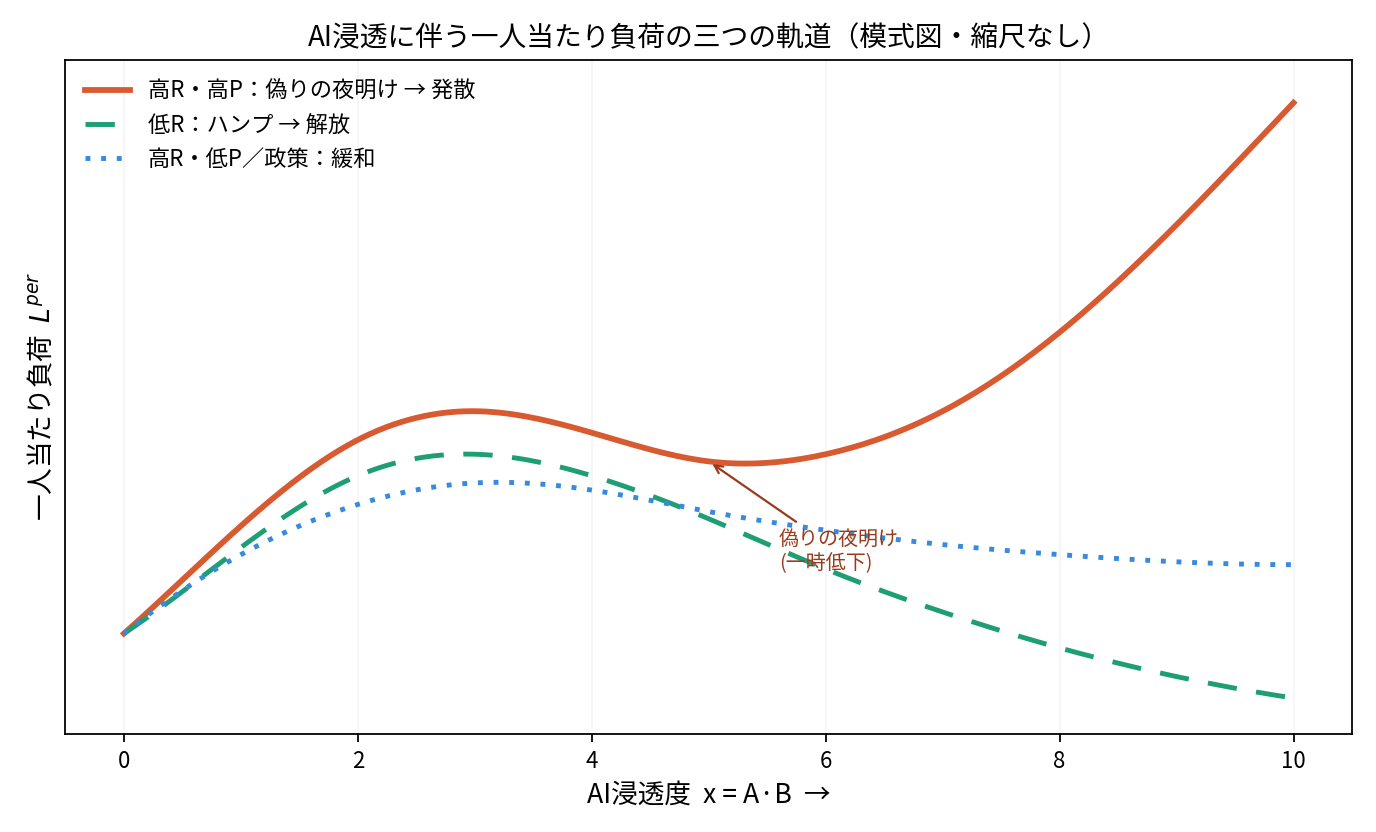
\includegraphics[width=0.86\textwidth]{figures/trajectory.png}
\caption{AI浸透に伴う一人当たり負荷の三つの軌道（\emph{模式図}。データに基づく推定ではなく、$\eta(x)$ の形状に関する仮定の下での図示）。高R高Pは中盤の「偽りの夜明け」の後に上限へ、低Rはハンプ後に低下、高R低P／政策介入は有界。}\label{fig:traj}
\end{figure}

\begin{cor}[技術だけでは負荷は下がらない]\label{c:policy}
$\delta(P)>0$ かつ $s_{\min}(R)>0$ の部門では、$x$ の上昇（純粋な技術改善）だけでは一人当たり負荷は低下しない。緩和の経路は命題\ref{p:margins}の(i)(ii)(iv)、すなわち (i) 責任の床 $s_{\min}(R)$ を下げる（定型案件のAI自己決裁を法的に許す）、(ii) 頭数弾力性 $\varepsilon_N(P)$ を上げる（有資格供給の拡大）、(iv) 賃金による調整を許す、のいずれかである。医師の働き方改革が「労働時間上限規制」という形をとるのは、床も供給も短期的に動かせないため、残る手段が $\bar T$ の直接規制だからと解釈できる。ただしこれは負荷を待ち行列へ振り替えるものであり、需要側の問題を解決しない。
\end{cor}

\subsection{$\Phi$--$\Psi$ 表記について：叙述上の要約とその限界}\label{sec:twoaxis}
本稿の四つの入力は、叙述の便宜上、二つのまとまりとして語ることができる。第一は浸透度 $x\equiv A\cdot B$ であり、これを\emph{適用可能性} $\Phi$ と呼ぶ（$A$ と $B$ はモデルを通じて積としてのみ現れる）。第二は $R$ と $P$ であり、いずれも「生成された生産性が単価や頭数へ逃げるのを妨げる」働きをもつため、まとめて\emph{制度的摩擦} $\Psi$ と呼ぶ。

\begin{rmk}[$L\propto\Phi\Psi$ という「会計恒等式」の撤回]\label{rmk:phipsi}
前版は $\Delta L^{\text{per}}\propto g(R)h(P)\,(A\cdot B)$ から $L^{\text{per}}\propto\Phi\cdot\Psi$ を導き、これを生産性の処分先を決める「会計恒等式」と呼んだ。この導出は成立しない。第一に、出発点である水準表現そのものを本稿は撤回している（注\ref{rmk:elasticity}）。第二に、微分的な応答の表現から水準の比例関係を導くことはできない。第三に、モデルにおいて $R$ は $\eta(x;R)$ を通じて、$P$ は $\varepsilon_N(P)$ を通じて入る\emph{別チャネル}であり、両者を一つのスカラー $\Psi=g(R)h(P)$ に束ねることは、$R$--$P$ 補完性という未検証の関数形仮定を先取りする。したがって $\Phi$ と $\Psi$ は\emph{叙述上の要約記号}であって、構造パラメータでも会計恒等式でもない。本稿の構造的な主張はすべて式\eqref{eq:master}に集約される。
\end{rmk}

\begin{rmk}[加法・乗法問題は未決のまま]\label{p:mult}
$\Psi=g(R)h(P)$ が $R$ と $P$ の積であるという仕様の下でのみ $\partial^2\Psi/\partial R\,\partial P>0$（$R$--$P$ 補完性）が成り立つ。第\ref{sec:measured}節で $R$ と $P$ が相関することは、この乗法仕様と\emph{両立的}ではあるが、それを\emph{識別するものではない}。説明変数間の相関（共線性）は、結果変数に対する両者の交互作用の関数形とは論理的に独立な情報である。加法／乗法の問い（H6）は未決であり、識別には一件あたり監督時間を結果変数とした $R\times P$ 交互作用項の直接推定（第8節 H6）を要する。
\end{rmk}

叙述上の要約として、$\Phi$ と $\Psi$ の高低による職業の四分類は表\ref{tab:phipsi}のようになる。これは\emph{定性的な整理}であって、モデルから導かれた分割ではない。

\begin{table}[h]\centering\small
\caption{$\Phi$（適用可能性）と $\Psi$（制度的摩擦）による定性的整理。モデルから導かれた分割ではなく叙述上の要約である。}\label{tab:phipsi}
\begin{tabularx}{\textwidth}{@{}lXX@{}}
\toprule
 & 摩擦 $\Psi$ 低 & 摩擦 $\Psi$ 高 \\ \midrule
適用可能性 $\Phi$ 高 & 生産性が\textbf{逃げる}：単価下落・再配置（翻訳、定型コード） & 生産性が\textbf{閉じ込められうる}：監督負荷または待ち行列（医療、監査、税務）。ただし系\ref{c:knife}の条件が同時に満たされる場合に限る \\[2pt]
適用可能性 $\Phi$ 低 & ほぼ変化なし（対人・現場） & 生産性が生成されず変化なし（介護・保育の身体介助） \\
\bottomrule
\end{tabularx}
\end{table}

\begin{figure}[t]\centering
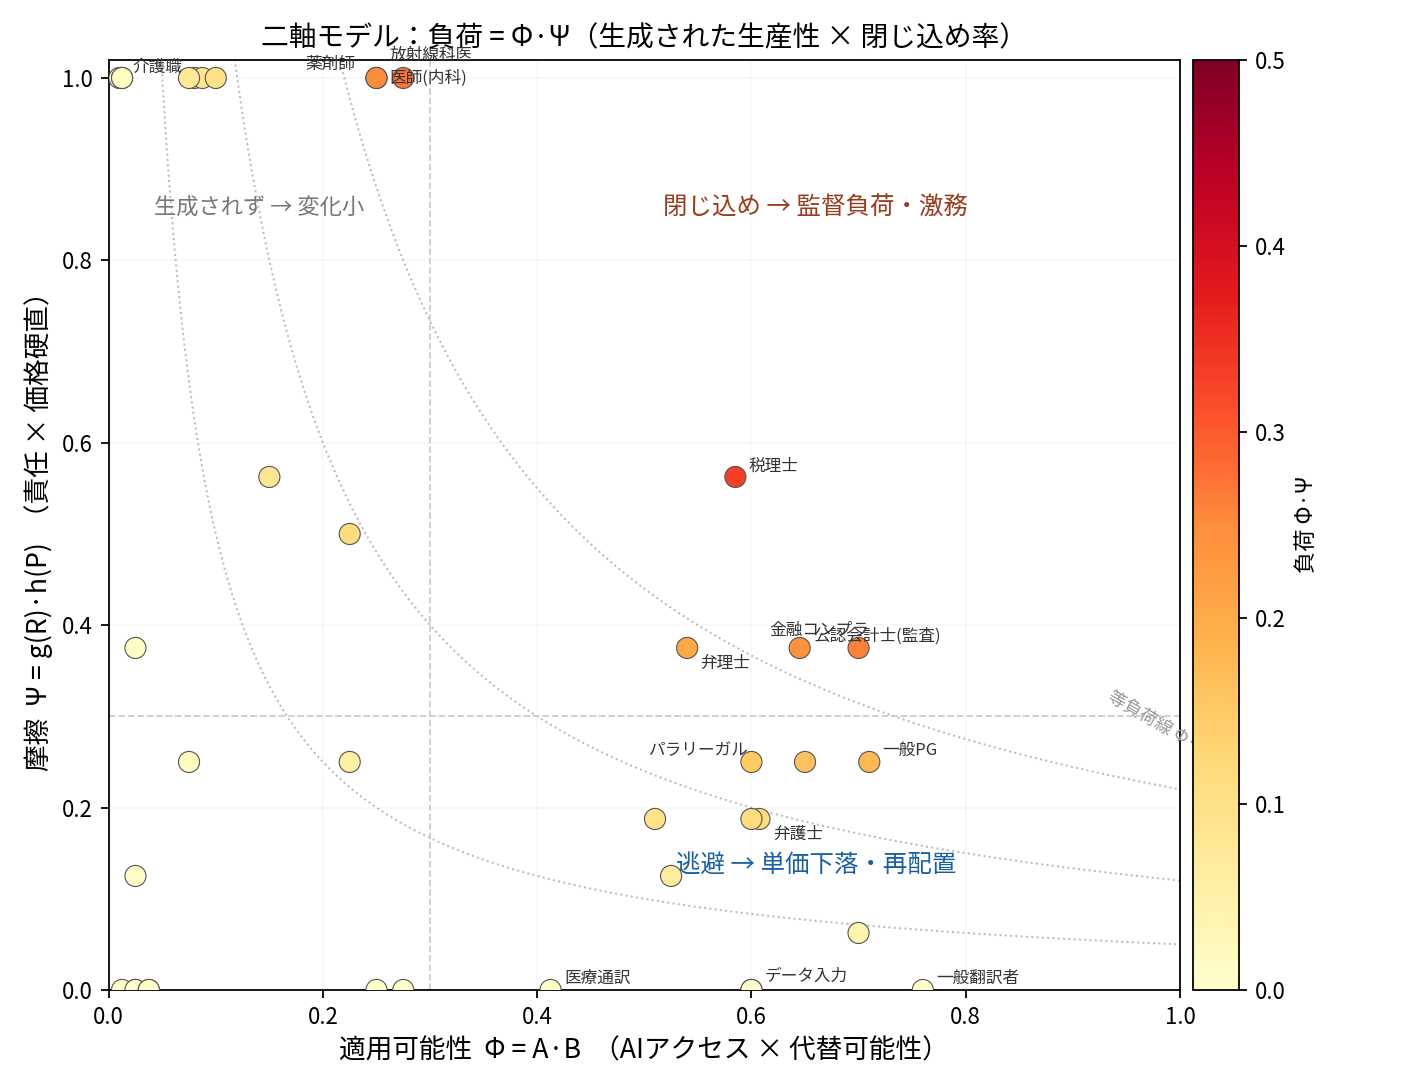
\includegraphics[width=0.82\textwidth]{figures/phipsi.png}
\caption{$\Phi$--$\Psi$ 平面上の職業分布（実測 $P$・$A$ 代理を使用）。点線は $\Phi\Psi=\text{const}$ の等高線だが、注\ref{rmk:phipsi}の通りこれは負荷の水準を表すものではなく、\emph{二つの要約軸の視覚化}に留まる。}\label{fig:phipsi}
\end{figure}

\begin{rmk}[記述的集約と介入的独立性の区別]
四変数が記述的に二つのまとまりとして語れることは、介入においても二つであることを意味しない。政策は\emph{素の四変数}に作用する：$A$ はアクセス政策、$B$ は「AIに何を委ねてよいか」の規制（自己決裁の許容範囲）、$R$ は責任法制、$P$ は価格自由化。$A$ と $B$ が高く相関していても、$B$ を動かす（AIに一次決裁を許す＝床 $s_{\min}$ を下げる）ことと $A$ を動かす（アクセス拡大）ことは別のレバーである。したがって四変数は、記述では冗長でも\emph{介入では独立な政策手段}として保持する。
\end{rmk}

\section{デジタルAIとフィジカルAI}

代替可能性 $B_j$ は一枚岩ではない。法務・会計・翻訳・プログラミング・調査・資料作成のように対象がデジタル情報で完結しやすいタスクでは、生成AIの効果は急速に現れる。これをデジタルAIによる代替可能性 $B_j^{D}$ と呼ぶ。一方、介護・建設・飲食・清掃・物流・医療現場・保育・警備のように、身体性・空間認識・手先の器用さ・人間との近接安全・予測不能な環境への即応が必要な仕事では、フィジカルAIによる代替可能性 $B_j^{P}$ が問題となる。両者を重み $\lambda_D,\lambda_P$ で合成する：
\begin{equation}
B_j=\lambda_D B_j^{D}+\lambda_P B_j^{P},\qquad
B_j^{P}=(\text{technical capability})\times(\text{environment fit})\times(\text{safety feasibility}).
\end{equation}
この分解により、ホワイトカラーとブルーカラーを硬い二分法ではなく連続的なグラデーションとして扱える。看護師は医療記録・問診整理・投薬確認ではデジタルAIの影響を受けるが、患者の移乗・表情変化の察知・緊急時対応ではフィジカルAIの制約を受ける。

資本主義的意思決定の下では、ヒューマンエラーの期待損失が大きい領域ほど代替圧力が高まる。企業は人間の賃金だけでなく、事故・訴訟・保険・評判毀損・品質ばらつきの期待コストを考慮する。したがって人間的な即応能力が価値をもつ場面でも、その価値への支払意思が弱く、AI・ロボットの総期待コストが十分低ければ置換が進む：
\begin{equation}
\text{置換が起きる} \iff C_{\mathrm{AI}}+E_{\mathrm{AI}}+R_{\mathrm{AI}}<C_{\text{Human}}+E_{\text{Human}}+R_{\text{Human}},
\end{equation}
ここで $C$ は直接費用、$E$ は誤り・事故の期待損失、$R$ は責任・保険費用である。フィジカルAIは環境適合性と安全性に制約されるが、$E_{\text{Human}}$ が大きい現場ほど投資が加速し、技術制約が突破された瞬間に急速な置換が生じうる。

\section{職業類型への適用}

\begin{table}[h]\centering\small
\caption{職業別の予測（定性）}\label{tab:occ}
\begin{tabularx}{\textwidth}{@{}lccccX@{}}
\toprule
職業領域 & $A$ & $B$ & $R$ & $P$ & 予測される再編 \\ \midrule
法務 & 高 & 高 & 高 & 低-中 & AIレビュー拡大。弁護士は監督・交渉・説明責任へ再編されるが、報酬自由化（$P$ 低）ゆえ単価圧力も併存する（医療との対照は\S\ref{sec:lawyer-med}）。 \\
医療 & 中-高 & 中-高 & 非常に高 & 非常に高 & 診断支援・記録自動化。責任は医師に残り監督負荷が増える。 \\
会計・監査 & 高 & 高 & 高 & 高 & 定型処理は自動化。監査判断・例外処理・署名責任が残る。 \\
翻訳 & 非常に高 & 非常に高 & 低 & 低 & 単価下落とポストエディット化。上位専門分野は残存。 \\
ソフトウェア開発 & 高 & 高 & 中 & 中 & コーディング高速化。要件定義・設計・責任ある運用へ価値移転。 \\
教育 & 中-高 & 中-高 & 中-高 & 高 & 教材作成・個別支援が増加。教師は伴走・評価・社会化支援へ。 \\
介護・保育 & 低-中 & 低-中 & 高 & 高 & 記録・見守りはAI化。身体介助・信頼形成は残存（ロボット性能次第）。 \\
物流・倉庫 & 中-高 & 中-高 & 低-中 & 低-中 & 標準環境ではロボット化。例外対応・保守へ人間が移る。 \\
\bottomrule
\end{tabularx}
\end{table}

法務領域は右上象限の典型である。AIによる契約レビュー・法令調査の代替可能性は高いが、資格・説明責任・守秘義務・利益相反管理・紛争時責任は残る。したがってAI導入は弁護士の消滅よりも、低位の調査・草案作成から高位の監督・判断・対人交渉への再配置をもたらす。AIが大量の案件を入口で拾い上げるなら、最終確認のボトルネックはむしろ強まる（命題\ref{p2}）。

医療領域も同様だが責任制約はさらに強い。AIが画像診断・問診要約・診療記録・薬剤相互作用チェックを支援しても、患者への説明と治療方針の責任は医師に残る。需要が拡大し患者側の期待水準が上がり説明義務が増えれば、単価が制度的に固定されるほど現場負荷は高まる（命題\ref{p3}）。

\paragraph{法務と医療の対照（$R$ 共有・$P$ 相違）.}\label{sec:lawyer-med}
弁護士と医師はともに $R$ が高いが、$P$ は大きく異なる。弁護士報酬基準は2004年に廃止され価格は自由化されており（実測 $P\approx1$、第7.3節）、診療報酬は全国一律の公定価格に固定される（実測 $P\approx4$）。本稿の枠組みは、この差が調整経路の差として現れると予測する：弁護士では監督への再編は起こりつつも単価圧力が併存しうる（命題\ref{p1}的要素が残る）のに対し、医師では単価チャネルが完全に閉ざされ負荷が処理件数・監督時間へ集中的に転嫁される（命題\ref{p3}）。表\ref{tab:jp}の一人当たり受任件数が横ばい〜微減にとどまる一方、医師の検査・診療負荷が高止まりする対比は、この予測と整合的である。両者は $R$ を一定に保ったまま $P$ が異なる、本稿の枠組み内での自然な準実験的対照をなす。

翻訳は対照的である。文章変換タスクの代替可能性は極めて高く、一般文書では $R$・$P$ がともに低い。この場合AIによる供給能力増加が単価下落として現れやすい（命題\ref{p1}）。ただし法務翻訳・医療翻訳・文学翻訳・ブランド文脈翻訳のように責任や文化的価値が高い部分では監修者としての人間需要が残る。

ソフトウェア開発では、AIはコード生成・テスト作成・バグ修正・ドキュメント作成を大きく補完する。しかし本番障害・セキュリティ・アーキテクチャ判断・顧客要件・組織内調整の責任は残る。結果として、コードを書く人間の価値は低下する一方、仕様を決めAI生成物を統合し障害責任を負う人間の価値は上がりうる。

\section{予備的実証分析}\label{sec:emp}

本章は理論モデルの\emph{予備的・記述的}検証である。本格的な因果推定は今後の課題とし、ここでは公開データに基づく記述統計と職業横断比較を行う。すべての日本側数値は出典に基づく概数または公開報告書からの近似値であり、本稿独自の調査ではないことを明記する。以下で示すのは「命題と整合的なパターン（stylized facts）」であって、命題の検証ではない。

\paragraph{なぜ職業\emph{横断}の記述分析なのか.}
記述分析という選択は、資源制約からの妥協であると同時に、対象そのものの性質に対応している。第\ref{sec:hours}節で見た通り、労働時間を結果変数とする最良の因果研究（Jiang et al., 2025）においてすら、係数は職業固定効果を入れると約6割低下し有意性を失いかける。すなわち\emph{識別変動の大半は職業間の横断差にあり、職業内の時系列変動ではない}。本稿の説明対象——責任制約 $R$ と価格硬直性 $P$——はまさにその職業間差であり、職業固定効果はそれを定義上すべて吸収してしまう。したがって、職業内の時間変動に依拠する標準的な差の差設計は、本稿の中心変数を推定できない。本稿が職業横断の比較と較正に向かうのはこのためである。この設計の代償は交絡の統制が弱いことであり、それを補うのが第\ref{sec:natexp}節の制度変化事例と第\ref{sec:survey}節の直接測定である。

\subsection{データソースと変数構成}
四変数を次の公開データから操作化する。$A$ は職業別AI利用率の代理として McKinsey Global Institute (2023, 2024)・OECD (2023)、国内では総務省「通信利用動向調査」を参照する。$B$ は Eloundou et al.\ (2024) のGPT曝露スコア（$\alpha,\beta,\zeta$ 指標）と Felten--Raj--Seamans (2023) のAIOEスコアを用いる（いずれも職業別値を公開）。$R$ は業務独占資格の有無・署名義務・訴訟リスク水準・EU AI Act 高リスク分類該当性から成る定性スコア（0--4）として補論Bのコードブックに従い付与する。$P$ は公定価格（診療報酬・介護報酬）・長期契約割合・価格分散の低さから推定する。

\begin{table}[h]\centering\small
\caption{変数の操作化に用いる主要データソース}\label{tab:src}
\begin{tabularx}{\textwidth}{@{}lXl@{}}
\toprule
変数 & 主要データソース & 近似値の典型範囲 \\ \midrule
$A$ & McKinsey GenAI Survey (2024); OECD Employment Outlook (2023); 総務省ICT統計 & 企業利用率 30--70\%（業種差大） \\
$B$ & Eloundou et al.\ (2024) GPT exposure; Felten--Raj--Seamans (2023) AIOE; O*NET tasks & 高曝露職 0.7--1.0、低曝露職 0.0--0.2 \\
$R$ & 本稿コードブック(補論B); 業種法令; EU AI Act Annex III & スコア 0--4 \\
$P$ & 中医協 診療報酬体系; 公認会計士監査報酬; 日本翻訳連盟 単価調査 & 硬直度: 医療$\approx$1, 翻訳$\approx$0.1 \\
\bottomrule
\end{tabularx}
\end{table}

本稿で扱う「実証」は記述統計と職業横断比較に限られる。因果推定（差の差分析、政策変更の自然実験）は第8節で論じる。$R$・$P$ は本稿著者による主観コーディングであり、再現性確保のため独立評価者による別途検証を要する点を強調しておく。

\subsection{ゴー/ノーゴー診断と $R$--$P$ 共線性}\label{sec:gonogo}
本格分析に入る前に、本稿の中心命題が乗る\emph{右上セル（高 $B$ × 高 $R$）が経験的に充足されているか}を点検する。これは安価な探索的事前点検である。補論Bの決定木コードブックを 39 職業（空間を張るよう選定、非対角セルを意図的に含む）に\emph{機械的に}適用し、$B$ を Eloundou 曝露（既知値）または推定値、$R$・$P$ を決定木スコアとして付与した。図\ref{fig:scatter}に $(B,R)$ 分布を示す（点の色が $P$）。本診断は\emph{第一次・単一コーダー}による暫定値であり、第8節の評価者間検証の対象である。

\begin{figure}[t]\centering
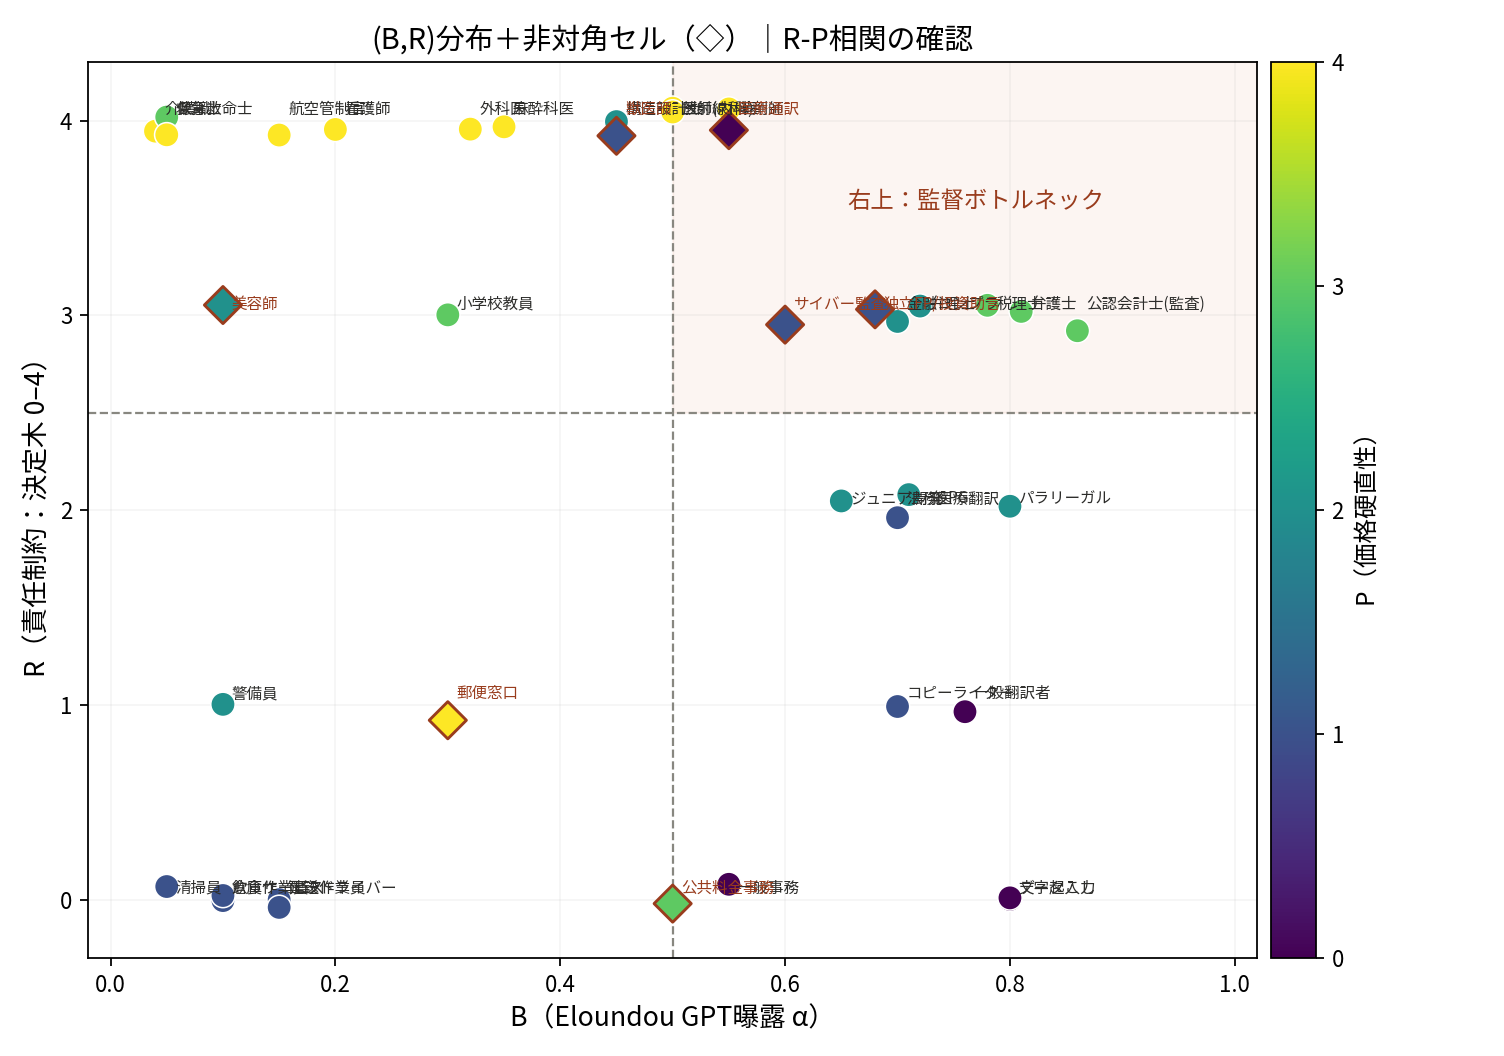
\includegraphics[width=0.92\textwidth]{figures/scatter.png}
\caption{$(B,R)$ 空間での職業分布。色は $P$（価格硬直性）。◇は非対角セルを埋めるため意図的に追加した職業。右上の網掛けが監督ボトルネック・セル。第一次・単一コーダーによる暫定コード。}\label{fig:scatter}
\end{figure}

二つの所見が得られた。第一に\textbf{（ゴー）}、高 $B(\ge0.5)$ × 高 $R(\ge3)$ のセルには 11 職業が分布し（弁護士・医師・放射線科医・薬剤師・公認会計士・税理士・弁理士・金融コンプライアンス等）、中心命題は検証に足る質量をもつ。第二に\textbf{（要注意）}、$R$ と $P$ が強く相関する。対角的な便宜標本では $r\approx0.91$、非対角セル（高 $R$・低 $P$：獣医師・医療通訳・独立投資助言・サイバー監査／低 $R$・高 $P$：公共料金事務・郵便窓口）を加えると $r\approx0.62$ に低下した。これは社会が\emph{責任の重い領域でこそ価格を規制する}ために生じる実質的相関であり、便宜標本の高い相関の一部はサンプリング由来である。

この共線性は本稿の枠組みにとって重要な含意をもつ。$R$ と $P$ が横断的に相関する以上、職業\emph{横断}比較では「$R$ の効果」と「$P$ の効果」を識別できない。したがって両者の分離は、\emph{職業内}の価格規制変動（同一 $R$ の下で保険診療と自由診療が併存する医療、独占資格者と隣接非資格者が混在する法務隣接領域）を利用する識別戦略に依存しなければならない。これは第8節 H5 の自然実験設計を、横断比較に対して優先すべき理由を強める。

\begin{rmk}[診断が露呈したコードブックの欠陥]
決定木の適用過程で、業務独占免許をもつが責任が軽い職業（例：美容師）が $R=3$ と過大評価される問題が判明した。原因は $R$ の Q1 が「免許の有無」のみを問う点にある。第8節の評価者間検証に先立ち、Q1 を「免許あり\emph{かつ}誤りが法的責任を生む」へ精緻化する（補論B 改訂）。測定の事前デバッグが本格コーディング前に欠陥を捕捉した一例である。
\end{rmk}

\begin{rmk}[予備的なAI補助評価者間信頼性検証]
本節の「第一次・単一コーダー」という限定を部分的に解消するため、独立4セッション（同一モデル系統3・別モデル系統1、いずれも本稿の仮説を与えないブラインド条件、$n=39$、線形重み付き Cohen's $\kappa$）による予備的なAI補助コーディングを実施した。結果、$R$ は著者-AI間で $\kappa=0.34$--$0.74$（同一モデル系統内では実質的一致だが、モデル系統をまたぐと「まずまず一致」まで低下）、$P$ は著者-AI間で $\kappa=0.43$--$0.62$（中程度一致）であった。モデル系統間の比較により、決定木の $R$ の Q4（「生命・身体・重大権利に直接関わるか」）が、(i) 従事者本人の労働災害リスクと第三者被害リスクの混同、(ii) 「重大権利」を財産権・手続き上の不利益まで広く読むか生命身体に限定して読むかという二重の解釈の余地をもつことが判明し、Q4を「従事者本人の労働災害リスクは含めない」「金銭賠償等で回復可能な損害は含めない」という除外規定つきで改訂した（補論B）。$P$ については決定木のQ3選択肢が雇用労働者の賃金決定メカニズムを明示的に扱っていない設計上のギャップも判明した。これらはAI(4セッション、2モデル系統)のみによる予備結果であり、人間コーダーによる検証(実施中)が本来の主要な証拠である。単一モデル系統のみでのクロスチェックは、系統間比較で初めて可視化される曖昧さを見落とし頑健性を過大評価しうる、という方法論的含意も得られた。
\end{rmk}

\subsection{実測 $P$ による妥当性検証と因子構造}\label{sec:measured}
$P$ の主観コーディングへの最大の批判を封じるため、$P$ を\emph{実測}に置換できる職業について公開データから規制シェア $M1$（売上に占める公定価格のカバー率）を構成した（出典は補論E）。医療は国民医療費（約45--47兆円）が全額保険診療であり、自由診療の中核である美容医療市場は2024年で約6{,}310億円（矢野経済研究所）に過ぎないため、規制シェアは約97\%と算定される。翻訳は公定価格をもたず、JTF『翻訳白書』の価格帯（和訳で19--22円が最頻だが MTPE の5--10円から目安26円超まで広く分散）から価格分散は大きい。表\ref{tab:measP}に主要職業の実測 $P$ を示す。

\begin{table}[h]\centering\small
\caption{実測 $P$（公定価格カバー率 $M1$ と価格分散）}\label{tab:measP}
\begin{tabularx}{\textwidth}{@{}lccX@{}}
\toprule
職業 & 規制シェア $M1$ & 実測 $P$ & 根拠（出典は補論E） \\ \midrule
医師・放射線科医・薬剤師 & $\approx0.95$--$0.98$ & 4 & 診療報酬・調剤報酬は全国一律の公定価格 \\
介護職・保育士 & $\approx0.85$--$0.90$ & 4 & 介護報酬・公費（一部自費） \\
航空管制官・郵便窓口 & $\approx0.95$--$1.00$ & 4 & 公務／認可料金 \\
タクシー運転手 & $\approx0.95$ & 4 & 道路運送法の認可運賃（低 $R$・高 $P$ の対照） \\
公認会計士（監査） & $\approx0.10$ & 2 & 監査報酬は交渉制だが慣行で粘着 \\
弁護士 & $\approx0.05$ & 1 & 弁護士報酬基準は2004年廃止・自由化 \\
翻訳者・データ入力 & $0.00$ & 0 & 公定価格なし・価格分散大 \\
\bottomrule
\end{tabularx}
\end{table}

三つの所見が得られた。第一に、\textbf{主観 $P$ は実測 $P$ でおおむね再現された}（重なる11職業で $r=0.90$、平均絶対差0.36）。とくに本稿の核心であるケーススタディ（医療＝高 vs 翻訳＝低）は実測でも保持される。第二に、実測 $P$ は\textbf{主観コーディングの系統的バイアスを補正した}。弁護士（主観 $P=3\to$ 実測1）と公認会計士（$3\to2$）で過大評価が判明した。原因は明確で、弁護士報酬基準は2004年に廃止され価格が自由化されている。「専門サービスは価格が粘着的」という事前観念が誤っていた。第三に、この補正は弁護士を高 $R$・低 $P$ セルへ移すため、$R$--$P$ 共線性をさらに緩めるはずだが、$r(R,P)$ は実測置換後も $0.62\to0.61$ とほぼ不変であった。\textbf{$R$--$P$ の相関（約0.6）はコーディング由来ではなく実質的である}。これは第7.2節の結論（横断分離は困難、識別は職業内 $P$ 変動による）を補強する。

\paragraph{相関構造。}最後に、四変数 $A,B,R,P$ が単一次元（「AI曝露の言い換え」）に潰れないかを点検する。$A$ は業種別生成AI導入率の代理（JUAS『企業IT動向調査2025』で社会インフラ60.8\%・金融保険54.4\%等、情報通信白書、PwC調査に基づく粗いマッピング）として39職業に付与した。標準化後の相関行列の固有値は $[2.20,\,1.37,\,0.29,\,0.13]$ であり、Kaiser 基準による成分数は2、累積寄与率は89.3\%である。したがって少なくとも、枠組みが単一の「AI曝露」次元へ還元されるわけではない。

前版はここで「$A$ と $B$ が一方の構成概念に、$R$ と $P$ が他方に負荷し、両者は\emph{直交する}」と述べたが、これは\textbf{報告した相関の選択に依存する誤った要約であり、撤回する}。表\ref{tab:corr}に全6組の相関を示す。

\begin{table}[h]\centering\small
\caption{$A,B,R,P$ の全対相関（$n=39$、$P$ は実測置換後）。前版は $r(B,R)$ のみを根拠に二軸の「直交性」を主張したが、$P$ は $A$・$B$ と中程度に相関する。}\label{tab:corr}
\begin{tabularx}{\textwidth}{@{}lcX@{}}
\toprule
組 & 相関係数 & 備考 \\ \midrule
$r(A,B)$ & $+0.861$ & 高い。高代替可能性タスクでこそAIアクセスが整備される内生的共起 \\
$r(R,P)$ & $+0.608$ & 中程度。責任の重い領域でこそ価格が規制される実質的相関 \\
$r(A,R)$ & $+0.015$ & ほぼ無相関 \\
$r(B,R)$ & $-0.016$ & ほぼ無相関（\emph{前版が「直交」の根拠としたのはこの1組のみ}） \\
$r(A,P)$ & $\mathbf{-0.405}$ & \textbf{中程度の負相関。前版は報告していない} \\
$r(B,P)$ & $\mathbf{-0.375}$ & \textbf{中程度の負相関。前版は報告していない} \\
\bottomrule
\end{tabularx}
\end{table}

\begin{figure}[t]\centering
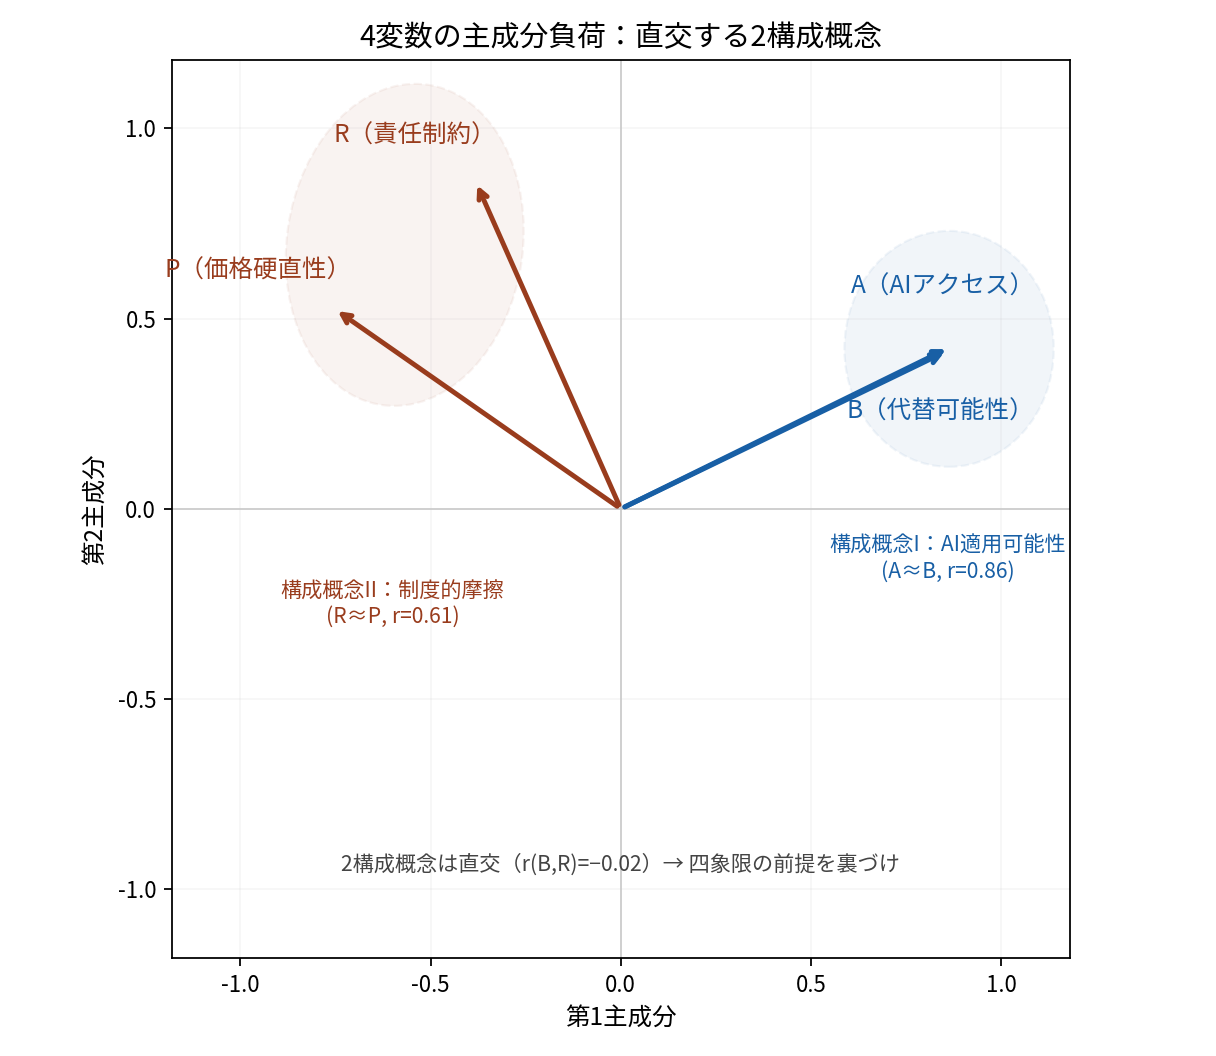
\includegraphics[width=0.72\textwidth]{figures/loadings.png}
\caption{$A,B,R,P$ の主成分負荷。前版はこの図を「二つの直交する構成概念」の証拠としたが、$P$ は第1・第2主成分の双方に実質的に負荷しており（本文参照）、$(A,B)$ と $(R,P)$ への清潔な分離は支持されない。}\label{fig:load}
\end{figure}

\begin{rmk}[「直交する二構成概念」の撤回]\label{rmk:pca}
三つの理由で、前版の解釈は維持できない。
\begin{enumerate}[label=(\roman*),leftmargin=1.8em,itemsep=1pt]
\item \textbf{報告の選択}。$B$ と $R$ がほぼ無相関であることは事実だが、$P$ は $A$（$-0.41$）とも $B$（$-0.38$）とも中程度に相関する。$r(B,R)\approx0$ の1組のみを根拠に二つのまとまりの「直交性」を主張することはできない。
\item \textbf{負荷の交差}。主成分負荷を見ると、$P$ は第1主成分に $+0.75$、第2主成分に $+0.53$ と\emph{双方に実質的に負荷}する。第1主成分は $A,B$（ともに $-0.86$ 前後）と $P$ を反対符号で対比する軸であり、第2主成分は $R$（$+0.86$）が支配する。すなわち経験的な布置は「適用可能性 vs 規制の対比軸」と「責任軸」であって、想定された $\Phi=(A,B)$／$\Psi=(R,P)$ の分離ではない。
\item \textbf{主成分の直交性は数学的性質である}。主成分どうしが直交することはPCAの構成上の帰結であり、潜在的な構成概念や政策手段が独立であることの実証的証拠ではない。
\end{enumerate}
したがって本稿が主張しうるのは、\emph{探索的に二つの相関クラスターが観察される}（$A$--$B$ が強く、$R$--$P$ が中程度にまとまる）ところまでであり、それ以上ではない。$n=39$ の便宜標本・単一コーダーによる序数コーディングという条件も、この分析の位置づけを探索的なものに留める。
\end{rmk}

\subsection{職業横断: $B\times R\times P$ と労働負荷}
表\ref{tab:cross}は主要専門職について Eloundou et al.\ (2024) のGPT曝露 $\alpha$ を $B$ の代理、補論Bに基づく $R$・$P$ スコア、公開統計から得られる労働強度指標を並べたものである。

\begin{table}[h]\centering\small
\caption{主要職業の GPT 曝露・$R$・$P$ スコアと労働強度指標}\label{tab:cross}
\begin{tabularx}{\textwidth}{@{}lcccX@{}}
\toprule
職業 & GPT曝露 $\alpha$ & $R$ & $P$ & 労働強度指標（出典） \\ \midrule
弁護士 (US: Lawyers) & 0.81 & 4 & 1$^{*}$ & 一人当たり民事訴訟受任件数: 横ばい〜微減（日弁連「弁護士白書」） \\
医師 (US: Physicians; JP: 医師) & 0.50--0.72 & 4 & 4 & 日本: 月80h超残業医師$\approx$30\%（厚労省検討会資料、改革前） \\
公認会計士 (Accountants) & 0.86 & 3 & 3 & 繁忙期90h超残業の常態化（金融庁・JICPA各種報告） \\
翻訳者 (Translators) & 0.76 & 1 & 0 & 単価: 英日で7--23円/ワード（2020年度JTF調査の分布）。MTPE案件は人間翻訳を下回る水準。時系列比較は未実施（注\ref{rmk:jtf}） \\
プログラマー (Software dev.) & 0.71 & 2 & 2 & Copilot利用者で工数 $-55.8\%$（Peng et al.\ 2023） \\
介護職 (Care workers) & 0.04 & 3 & 4 & 人手不足深刻、有効求人倍率 $\approx4$ 倍（厚労省） \\
倉庫作業員 (Warehouse) & 0.05--0.20 & 1 & 1 & 自動化拡大、事故率はロボット導入後上昇報告も \\
\bottomrule
\end{tabularx}
\end{table}

\noindent 注: GPT曝露 $\alpha$ は Eloundou et al.\ (2024) Table 1 および公開リポジトリ値の近似。$R$・$P$ は補論Bに基づく主観コーディング。労働強度指標は各出典の概数による定性記述。$^{*}$弁護士の $P$ は主観コーディングでは3だったが、報酬基準が2004年に廃止・自由化された事実に基づく実測値（第7.3節）に置き換えている。

\smallskip
表\ref{tab:cross}から次のパターンが\emph{読み取れる（因果ではなく、また命題の検証でもない）}。第一に、翻訳者は $\alpha$ が高い（0.76）一方 $R,P$ がともに低く、業界では単価下落が広く認識されている。方向としては命題\ref{p1}と整合的だが、時系列的な確認は取れていない（注\ref{rmk:jtf}）。第二に、医師・会計士は $\alpha$ が高く $R$・$P$ がともに高い一方、弁護士は実測 $P=1$ であり高 $R$・低 $P$ に位置する（\S\ref{sec:lawyer-med}）。労働強度指標は医師・会計士で高止まりし、弁護士では横ばい〜微減である。この差は $P$ チャネル（命題\ref{p3}）の予測方向と整合的だが、\emph{これらの水準はいずれも生成AI普及以前から続く状態であり、AI起因の変化を示すものではない}（第\ref{sec:trend}節）。第三に、介護職は $\alpha$ が極端に低く（0.04）$R$・$P$ は高いが $x$ が低いため、本稿の機構は作動せず、人手不足という別の要因が支配的である。

\subsection{ケーススタディ: 翻訳市場 vs 医療市場}
命題\ref{p3}を、価格構造が対照的な二市場で対比する。

\subsubsection{翻訳市場（低$R$・低$P$）}
翻訳市場は典型的なスポット市場である。MTPE (Machine Translation Post-Editing) が標準化し、機械翻訳を前提とした案件の単価は人間翻訳を大きく下回る水準で定着したとされる。これは命題\ref{p1}（$x$ 高、$R$・$P$ 低）の予測方向と整合的である。法務・医療・文学翻訳では $R$ がやや高くなるため価格下落は限定的で「上位市場への退避」が観察される。

\begin{rmk}[単価データに関する重要な留保]\label{rmk:jtf}
本稿は当初、英日翻訳の単価が「2010年頃 1字当たり20--25円から2018年以降5--10円へ下落した」と記述していたが、この記述は次の二つの問題を含むため撤回する。
\begin{enumerate}[label=(\roman*),leftmargin=1.8em,itemsep=1pt]
\item \textbf{単位の誤り}。日本の翻訳業界では、英日翻訳は原文の\emph{英単語}あたり（円/ワード）、日英翻訳は原文の\emph{日本語文字}あたり（円/文字）で建値されるのが通例である。英日翻訳の単価を「円/字」と表記していたのは誤りである。
\item \textbf{出典の不足}。JTF『翻訳白書』の分野別単価詳細表は会員限定資料であり、本稿の範囲で一次確認できたのは公開記事に基づく単一年度（2020年度調査）の分布のみである（英日・翻訳会社経由で7--15円/ワード、ソースクライアント直で11--23円/ワード、日英・翻訳会社経由の最頻値帯が5--7円/文字）。2010年頃の水準は一次資料で確認できていない。
\end{enumerate}
したがって、NMT画期（2016--17年）および生成AI画期（2022年11月）をまたぐ傾きの比較は本稿では実施できていない。「翻訳単価が下落した」という業界の一般的認識と本稿の予測方向は一致するが、\emph{その時系列的な確認は今後の課題}であり、本節の記述は仮説の例解に留まる。
\end{rmk}

\subsubsection{医療市場（高$R$・高$P$）}
日本の医療市場は対照的に、診療報酬制度（中医協が定める公定価格）により価格硬直性が極めて高い。画像診断AI（Aidoc、富士フイルムCXR-AID、エルピクセルEIRL等）は2018年頃から導入が進むが、診療報酬上の評価は限定的である。一方でAI画像診断のための撮影・読影件数は増加しており、放射線科医の負荷は減らず、診療体制によっては増加する事例も報告される（日本医学放射線学会の各種講演・調査）。これは命題\ref{p3}の予測通り、価格硬直下では生産性上昇が単価ではなく処理件数として表面化する例である。本稿のモデルはこれを次のように説明する：診療報酬が固定（$P\approx1$）で医師の医療責任が法的に強固（$R$ 高）ゆえ、AI導入による一案件あたり費用低下は需要側（高齢化・検査基準）の拡大により件数増として吸収され、医師数の供給は医学部定員・専門医制度により短期非弾力的（$\varepsilon_N\approx0$）であるため一人当たり監督件数が上昇する。

\begin{rmk}[限界：NDBオープンデータによる定量検証はAI固有の加速を確認できなかった]
NDBオープンデータ（第1--10回、2014--2023年度、外来CT・MRI算定回数）による定量的検証では、2018年のAI画像診断承認開始を境にした傾きの加速は確認できなかった（CT傾き比0.89とむしろ鈍化、MRI傾き比1.14とごく僅かな加速）。生成AI画期（2022年11月）については、完全に画期後となる年度データが2023年度の1点のみであり、傾きの折れを判定すること自体ができない。したがって「AI画像診断導入後に検査件数が増加している」という本文の記述は事実として正しいが、これは2014年から一貫する高齢化・検査適応拡大の長期トレンドと区別できておらず、AI固有の加速効果を示す証拠ではない。これは本稿の記述分析の限界であり、部署・施設単位のAI導入時期差を用いた staggered DID（第8節 H2）を要する。
\end{rmk}

\subsubsection{二市場の対比と留保}
\begin{table}[h]\centering\small
\caption{翻訳市場と医療市場における AI 影響の対比}\label{tab:two}
\begin{tabularx}{\textwidth}{@{}lXX@{}}
\toprule
指標 & 翻訳市場 (低$R$・低$P$) & 医療市場 (高$R$・高$P$) \\ \midrule
価格調整 & 単価が約50\%低下 (2010$\to$2024 概算) & 診療報酬体系に固定、AI評価点未確立 \\
需要側反応 & 案件総数増、ポストエディット標準化 & 撮影・検査件数増、AI支援必須化 \\
労働者数 & 専業翻訳者は減少、ポストエディター増加 & 医師数微増（定員拡大）、専門医偏在 \\
一人当たり負荷 & 実質収入は減少、件数増 & 残業時間高止まり、月80h超約30\%（改革前） \\
制度反応 & 市場が自発調整（標準化） & 働き方改革2024年4月施行（労働時間規制） \\
予測との整合 & 命題\ref{p1}と整合 & 命題\ref{p3}と整合 \\
\bottomrule
\end{tabularx}
\end{table}

同じく高いAI曝露（$\alpha>0.5$）をもつ二職業が、$P$ と $R$ の組合せの違いによって正反対の市場反応を示すという事実は、従来のタスク代替論や曝露スコア\emph{単独}では説明しにくく、本稿の枠組みと\emph{整合的}である。ただしこれは観察された相関であって因果的証拠ではない。両市場は需要動学（高齢化 vs グローバル化）・規制環境・労働供給制度が大きく異なり、$P$ 以外の交絡を統制していない。

\subsection{先行技術による同型ケース：電子カルテと環境AI記録}\label{sec:ehr}
本稿のモデルにとって最も情報量の多い経験的素材は、生成AIそのものではなく、\emph{同じ制度条件の下で既に一巡した技術}である。米国外来医療は、公定的な診療報酬体系により単価が動かず（$P\approx1$）、医師数が資格制度により短期非弾力的で（$\varepsilon_N\approx0$）、記録の最終署名が医師に残る（$s_{\min}(R)>0$）という、本稿が指定する三条件をすべて満たす。ここで電子カルテ(EHR)と環境AI記録という二世代の技術が、順に観察可能な自然史を残している。

\paragraph{第一世代：電子カルテ（一巡した事例）.}
Sinsky et al.\ (2016) は4診療科57名の医師を430時間にわたり直接観察し、診療時間のうち\emph{患者との直接対面が 27.0\%、EHRと事務作業が 49.2\%} を占めることを示した。直接診療1時間あたり約2時間が記録・事務に費やされる計算である。効率化技術として導入されたEHRの下で、単価は動かず、医師数も大きくは増えず、負担は\emph{一人当たりの時間}として現れた。本稿の五マージンのうち、(i) 単価低下でも (ii) 頭数増でもなく (iii) 一人当たり時間増が作動した事例と読める。

ただし\emph{重要な非対称性}を明記しなければならない。EHRは一件あたり記録時間を\emph{削減しなかった}——むしろ記録要件の拡大を伴って増加させた可能性が高い。本稿の仮定\ref{a:tech}は $\partial s/\partial x\le0$、すなわち技術は一件あたり監督時間を減らす方向にのみ働くと置いている。したがってEHRは本稿の機構（$\delta>\eta$ による負荷増）の実例ではない。この事例が示すのは\emph{どのマージンが吸収したか}であって、$\eta$ の大きさではない。$P\approx1$・$\varepsilon_N\approx0$ の下では負担が時間へ向かうという\emph{振替先の予測}に対する傍証として扱うのが正確である。

\paragraph{第二世代：環境AI記録（進行中の検定）.}
環境AI記録（ambient AI scribe）は、この非対称性を解消する。診察音声から記録原案を自動生成するため、一件あたり記録時間を\emph{削減する}方向に働き、$\eta>0$ が成立する。近年の二つの大規模研究が、本稿の予測に対する事実上の検定を提供している（表\ref{tab:scribe}）。

Lukac et al.\ (2025) は 14 診療科・238 名の外来医師を三群（DAX、Nabla、通常診療）へ無作為割付し、約7.2万件の診察を2か月間追跡した。Nabla 群では一記録あたり時間が 4分30秒から3分49秒へ、対照比 9.5\% 減少した（DAX 群は有意でない）。すなわち $\eta>0$ は確認されるが、その大きさは一桁パーセント台である。同研究は「本技術は受動的な受容ではなく\emph{能動的な医師の監督}を要する」と結論しており、両プラットフォームで臨床的に重要な不正確さが時折観察されたことを報告している。これは責任の床 $s_{\min}(R)>0$ の直接的な記述である。

Rotenstein et al.\ (2026) は5つの学術医療センターにおいて、環境AI記録を採用した 1{,}809 名と非採用の 6{,}772 名を 2023--2025 年にわたり比較した。結果は本稿にとって決定的な形をしている：記録時間は日あたり 16 分（相対 10\%）減少し、EHR滞在時間も 13 分（同 3\%）減少した。しかし\emph{勤務時間外のEHR利用には有意な差がなく}、代わりに\emph{週あたり外来件数が約 0.5 件増加}した。

\begin{table}[h]\centering\small
\caption{環境AI記録の主要研究：一件あたり時間と一人当たり時間の乖離}\label{tab:scribe}
\begin{tabularx}{\textwidth}{@{}lXX@{}}
\toprule
 & Lukac et al.\ (2025), NEJM AI & Rotenstein et al.\ (2026), JAMA \\ \midrule
設計 & 無作為化試験、238名・14診療科・約7.2万診察、2か月 & 観察研究、採用1{,}809名 vs 対照6{,}772名、5施設、2023--2025 \\
一件あたり時間（$s$） & 記録時間 $-9.5\%$（Nabla）／有意差なし（DAX） & 記録時間 $-16$ 分/日（相対 $-10\%$） \\
一人当たり時間（$\ell$） & 測定対象外 & 勤務時間外EHR利用に\emph{有意差なし} \\
処理件数（$X$） & 測定対象外 & 週あたり外来 \emph{$+0.5$ 件} \\
責任の床 & 「能動的な医師の監督を要する」。不正確さを時折観察 & 署名義務は不変 \\
\bottomrule
\end{tabularx}
\end{table}

\paragraph{モデルによる読み.}
中核式\eqref{eq:master}の言葉でいえば、この組合せは $\eta>0$ かつ $\delta(P)\approx\eta$ の状態である。一件あたり監督時間は確かに減った（$\eta>0$）が、\emph{一人当たり時間としては現れず}、削減分はおおむね件数の増加として吸収された。$P\approx1$ ゆえ単価は下がりようがなく、$\varepsilon_N\approx0$ ゆえ頭数も増えない。残る調整先は件数と時間であり、観察されたのは前者への振替である。

ここで慎重を要するのは、これが\emph{負荷の増加の証拠ではない}ことである。$\ell$ は増えておらず、命題\ref{p3}が主張する $\delta>\eta$ は成立していない。本事例が実際に示すのは、より弱く、しかし本稿にとって十分に重要な次の一点である：\emph{高 $P$・低 $\varepsilon_N$ の環境では、一件あたりの時間短縮は一人当たりの時間短縮として現れない}。素朴な「AIは労働時間を減らす」という予測は、この設定では成立していない。これは第\ref{sec:counter}節が扱う低 $R$・低 $P$ 環境での結果（時間の減少・精密なゼロ）と正反対の吸収様式であり、制度条件によって振替先が変わるという本稿の中心的な主張と整合する。

\begin{rmk}[本事例に対する留保]
第一に、Rotenstein et al.\ (2026) は観察研究であり、採用の内生性（多忙な医師ほど採用する、あるいはその逆）を除去していない。第二に、週 0.5 件の増加が供給側の選択（余力を診療に充てた）か需要側の圧力（待機患者の消化）かは区別されていない。本稿のモデルは後者を想定するが、前者であれば厚生的な含意は逆になる。第三に、両研究とも\emph{バーンアウト指標は改善}を報告しており（Lukac et al.\ で約7\%）、負荷が主観的悪化として現れているわけではない。本稿のモデルは時間と件数を扱い主観的負荷を直接には扱わないため、この点は整合とも不整合とも言えない。第四に、いずれの研究も価格の外生変動を利用しておらず、$P$ の因果的役割は示されていない。$P$ の識別には第\ref{sec:natexp}節のような制度変化か、第8節 H2 の設計を要する。
\end{rmk}

\subsection{日本の専門職データから見る命題1・2・3}

\begin{table}[h]\centering\small
\caption{日本の主要専門職の労働市場指標（公開データに基づく概数）}\label{tab:jp}
\begin{tabularx}{\textwidth}{@{}lXccX@{}}
\toprule
職業 & 主要指標 & 2020年頃 & 2024年頃 & 出典・備考 \\ \midrule
弁護士 & 弁護士数（人） & 約42,200 & 約45,500 & 日弁連「弁護士白書」各年版 \\
 & 一人当たり民事訴訟受任件数 & 減少傾向 & 横ばい〜微減 & 同上（簡裁減、地裁横ばい） \\
医師 & 医師数（人） & 約34万 & 約34.7万 & 厚労省「医師・歯科医師・薬剤師統計」 \\
 & 勤務医 月80h超残業者比率 & 約30\% & 約20\%（改革後） & 厚労省「医師の働き方改革検討会」資料 \\
公認会計士 & 会計士数（人） & 約3.3万 & 約3.5万 & JICPA会員数統計 \\
 & 監査報酬総額 & 増加傾向 & さらに増加 & 金融庁監査人交代調査、業界レポート \\
翻訳者 & フリーランス専業者 & 減少 & さらに減少 & JTF業界調査・矢野経済研究所 \\
 & 英日翻訳単価（円/ワード） & \multicolumn{2}{c}{7--23（2020年度調査の分布）} & JTF公開記事。年次比較は未取得（注\ref{rmk:jtf}） \\
\bottomrule
\end{tabularx}
\end{table}

\noindent 注: 数値はすべて出典に基づく概数・近似値であり、本稿の独自推計ではない。

\begin{itemize}[leftmargin=1.4em,itemsep=2pt]
\item \textbf{命題\ref{p1}（低$R$・高$B$ $\Rightarrow$ 単価下落先行）}: 翻訳市場は単価下落と専業者減少を明瞭に示し、整合的。
\item \textbf{命題\ref{p2}（高$R$・高$B$ $\Rightarrow$ 監督増・雇用維持先行）}: 弁護士・医師・公認会計士はいずれも資格者総数が微増し、雇用は消滅していない。整合的。ただし一人当たり業務負荷の指標は職業によって分かれる：医師・公認会計士（高 $R$・高 $P$）では残業・繁忙期労働が高止まりする一方、弁護士（高 $R$・低 $P$、実測第7.3節）では一人当たり受任件数はむしろ横ばい〜微減である。これは負荷の集中が $R$ ではなく $P$ に依存するという命題\ref{p3}の予測と整合的であり（\S\ref{sec:lawyer-med}）、$R$ 単独では負荷の増減を説明できないことを示す。
\item \textbf{命題\ref{p3}（高$P$ $\Rightarrow$ 単価でなく件数で吸収）}: 医療の診療報酬はAI利用への点数評価が限定的なまま、画像検査・AI支援診断件数は増加。整合的。
\end{itemize}

\begin{rmk}[重要な交絡：医師残業の見かけの低下]
医師の月80h超残業者比率の低下（約30\%$\to$約20\%）は、一見すると命題\ref{p3}（負荷増）と\emph{矛盾}するように見える。しかしこの低下は2024年4月施行の働き方改革による\emph{外生的な時間上限規制}の効果が大きく、AI導入による負荷軽減効果とは切り分けられない。むしろ規制で残業の\emph{上限}が抑えられた一方、検査・問診・記載量という\emph{未処理マージン}は増え続けており、規制を統制した上での真の負荷を測るには差の差分析が不可欠である（第8節）。観察された残業低下を「AIが負荷を下げた証拠」と読むことは交絡により誤りうる。
\end{rmk}

\subsection{自然実験的な制度変化：不妊治療の保険適用（2022年）---$P$ チャネルの補助的事例}\label{sec:natexp}
第7.2節は、$R$ と $P$ が横断的に相関するため両者の分離には\emph{職業内}の価格規制変動が必要だと結論した。本節はその設計（第8節 H5）を実データで一本実行する。2022年4月、日本では体外受精・顕微授精等の生殖補助医療（ART）が\emph{自由診療から保険診療へ移行}した。これは同一の医療責任（$R$ 一定）の下で価格レジームのみが外生的に変化した稀有な自然実験である：価格は自由設定（$P\approx0$、施設ごとに分散）から全国一律の公定点数（$P\approx1$）へ転じ、患者負担は全額自己負担から3割へ低下した。本稿の $P$ チャネル（命題\ref{p3}）に対する補助的な観察機会を与える。\textbf{ただし本節はAIショックではなく価格規制の変化を用いており、AI起因の監督ボトルネック効果そのものを識別するものではない。}示せるのは「責任 $R$ を一定に保ったまま価格硬直 $P$ が高まると、調整が単価ではなく数量・負荷で起こる」という $P$ チャネルの整合性までである。

\begin{figure}[t]\centering
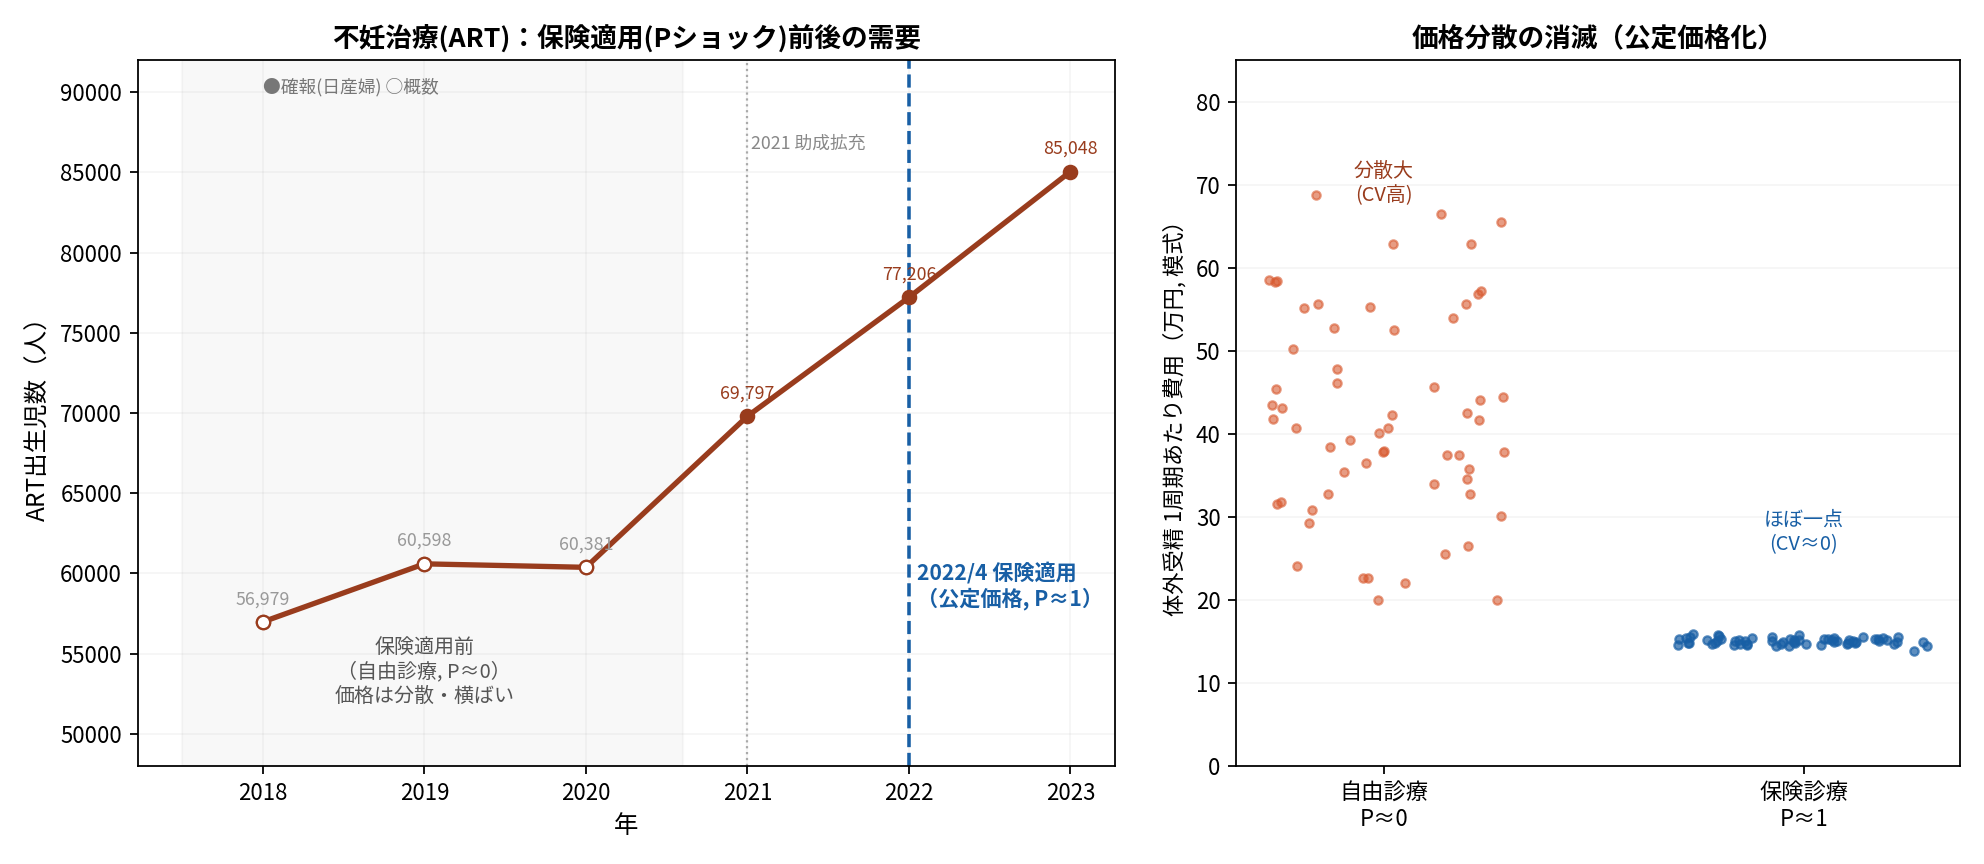
\includegraphics[width=0.98\textwidth]{figures/h5.png}
\caption{不妊治療の保険適用（2022年4月）を挟むART需要と価格分散。左：ART出生児数は保険適用前（2016--2020）に横ばいだったが、2021年の助成拡充・2022年の保険適用を経て急増（2020年約6.0万→2023年8.5万、$+41\%$、出典：日本産科婦人科学会ARTデータブック、2018--20は概数）。右：価格は自由診療下の広い分散から公定価格下のほぼ一点へ（模式図）。}\label{fig:natexp}
\end{figure}

命題\ref{p3}の予測どおり、四つの帰結が同時に観察される（図\ref{fig:natexp}）。第一に、\textbf{価格分散の消滅}。自由診療下では1周期あたり費用が施設ごとに大きく分散していたが（おおむね30--60万円台）、保険適用後は公定点数により全国でほぼ一点に収束した（$P$ の操作的定義そのもの）。第二に、\textbf{患者価格の低下}（全額$\to$3割）。第三に、\textbf{需要の急増}。ART総治療周期は2022年に過去最多の54万3{,}630件、2023年は56万1{,}664件（$+18{,}034$）へ、ART出生児数は2021年6万9{,}797人$\to$2022年7万7{,}206人$\to$2023年8万5{,}048人と3年連続で過去最多を更新した。第四に、\textbf{供給の非弾力性}。ART実施は認可・登録施設（約600施設）に限られ、生殖医療専門医プールも小さいため、件数増は短期的に施設・専門医あたりの処理負荷へ転化する（$\varepsilon_N\approx0$）。

これは命題\ref{p3}の中核——\emph{価格が硬直化（$P\uparrow$）すると、生産性・需要の拡大は単価ではなく件数として吸収され、非弾力的供給の下で一人当たり負荷へ転嫁される}——を、$R$ を一定に保ったまま示す。対照として、美容医療は同期間を通じて自由診療（$P\approx0$）に留まり、価格競争と広い価格分散を維持したまま市場が拡大した（2024年約6{,}310億円、矢野経済研究所）。同じ医療という $R$ 領域の内部で、$P$ の高低が「件数・負荷で吸収（ART）」と「価格競争（美容）」という正反対の調整を生む。これは $P$ チャネルの補助的な制度的証拠である（AI効果の識別ではない）。

単純な最小二乗法でトレンドの折れを定量化すると、ART出生児数の年間増加数は2001--2020年（保険適用前）の平均+2{,}845人/年から、2021--2023年には+7{,}626人/年へ約2.7倍に加速した（治療周期数は+24{,}118件/年から+31{,}832件/年へ約1.3倍）。これにより、保険適用前（2016--2020年）が実際には相対的に緩やかな増加にとどまっていたことが確認でき、2021年の助成拡充・2022年の保険適用による加速が既存トレンドからの明確な乖離であることが裏づけられる。

\begin{rmk}[この自然実験の限界]
四点を明示する。(i) 本実験が識別するのは $P$ チャネルであって、AI導入の効果ではない。AIショックではなく価格規制ショックを用いている。(ii) 2021年の助成拡充が2022年保険適用と時期的に近接し、需要増の寄与を完全には分離できない（純粋な保険効果の識別には月次データの回帰不連続が望ましい）。(iii) 一人当たり負荷は件数増と供給非弾力性から\emph{推論}しており、施設・医師あたり労働時間の直接観測ではない。(iv) これは公開集計を用いた中断時系列・記述的自然実験であり、施設パネルの差の差分析ではない。それでも、$R$ 一定下での外生的 $P$ 変動という設計上の強みにより、命題\ref{p3}の $P$ チャネルに対する最も直接的な証拠を与える。
\end{rmk}

\subsection{米労働市場への探索的適用（補論）}\label{sec:usmap}
二軸枠組み（$\Phi\times\Psi$）を LLM 採点ツールと規則ベース採点を用いて米労働市場全体（約1億4{,}300万人）へ試みに適用した探索的分析を補論Fに示す。用いるツールは本人が学術的精密出版物ではないと明示する公開可視化ツールであり、点推定（とくに監督ボトルネック雇用の比率が7\%--35\%という幅）ではなく、頑健な定性的順序――監督ボトルネックは高曝露雇用の少数派に集中し、多数派にはそれを守る摩擦が存在しない――のみを主張の対象とする。

\subsection{公開集計によるトレンド分析：生成AI固有の折れは検出されなかった}\label{sec:trend}
本節の記述分析に対する最も自然な批判は、\emph{示されている「負荷の高さ」がいずれも生成AI普及以前から続く慢性的な状態であり、AI起因の変化と区別できない}というものである。この批判に応えるため、公開集計から取得できた三系列について、画期の前後で傾きが変化したか（トレンドの折れ）を単純な最小二乗により点検した。結果は本稿にとって否定的であり、そのまま報告する。

\begin{table}[h]\centering\small
\caption{画期前後の傾き比較（公開集計による探索的分析）}\label{tab:trend}
\begin{tabularx}{\textwidth}{@{}lXX@{}}
\toprule
系列 & 画期前後の傾き & 判定 \\ \midrule
CT撮影件数（NDBオープンデータ、2014--2023年度、外来算定回数） & 2018年（AI画像診断承認開始）前 $+53.2$万件/年 $\to$ 後 $+47.5$万件/年（比0.89） & \textbf{加速なし}（むしろ鈍化） \\
MRI撮影件数（同上） & 同 $+27.0$万件/年 $\to$ $+30.9$万件/年（比1.14） & \textbf{ほぼ変化なし}（誤差の範囲） \\
ART出生児数（日本産科婦人科学会、2001--2023年） & 2021年前 $+2{,}845$人/年 $\to$ 後 $+7{,}626$人/年（比2.7） & \textbf{明瞭な折れ。ただし原因はAIではなく助成拡充・保険適用} \\
英日翻訳単価（JTF） & \multicolumn{2}{X@{}}{複数時点データを一次資料から取得できず、傾き比較は\textbf{実施不能}（注\ref{rmk:jtf}）} \\
\bottomrule
\end{tabularx}
\end{table}

三点を明記する。第一に、\textbf{生成AI画期（2022年11月）に固有のトレンド変化は、いずれの系列からも検出されなかった}。CT・MRIについては、画期後に完全に該当する年度が2023年度の1点のみであり、傾きの折れを判定すること自体ができない。第二に、唯一明瞭な折れを示したART系列の原因は、AIではなく2021年の助成拡充と2022年の保険適用という価格・制度ショックである（第\ref{sec:natexp}節）。第三に、したがって\emph{本節が示す「高 $R$・高 $P$ 職の負荷が高い」という記述は、生成AI以前から続く構造の持続と区別できていない}。これは冒頭の批判が現時点では妥当であることを意味する。本稿の枠組みを支持する時系列的証拠は、現時点では存在しない。

\subsection{AI適用率と需要吸収条件の職業別較正}\label{sec:aei}

前節までの記述分析は、負荷の\emph{結果}を公開集計で近似しようとして失敗した。本節は方向を変え、中核式\eqref{eq:master}の\emph{技術側パラメータ}を、AI利用の職業別公開集計（Anthropic Economic Index、以下AEI、CC-BY）を用いて較正する。本節は\textbf{モデルの検定ではなく、タスク側パラメータの較正と測定監査}である。

\subsubsection{推定対象}
測るのは職業全体の労働時間ではない。データ源 $d$（Claude.ai／Cowork、または 1P API）において\emph{観測されたタスク}について、AI支援下に残存する人間関与時間の比
\begin{equation}\label{eq:rho}
\rho_{jd}\;=\;\frac{\tilde T_{1,jd}}{60\,T_{0,jd}},
\qquad
\tilde T_1=\text{AI支援ありの推定所要時間（分）},\;
T_0=\text{AI無しの推定所要時間（時間）}
\end{equation}
である。ここで $\tilde T_1$ は\emph{監督時間そのものではない}。指示の作成、AIとの反復、人間自身による直接作業、情報収集、判断・承認がすべて含まれる合成量である。

\paragraph{推定対象の向き（潜在量と推定値を分ける）.}
まず\emph{潜在量}について述べる。残存人間関与時間 $\tilde s^{*}$ は、不可避な監督時間 $s^{*}$ とそれ以外の関与 $q^{*}\ge0$ の和
\[
\tilde s^{*}=s^{*}+q^{*}\;\ge\;s^{*}
\]
であるから、必要需要倍率についても
\[
M^{*}_{\mathrm{res}}=\frac{T_0^{*}}{\tilde s^{*}}\;\le\;\frac{T_0^{*}}{s^{*}}=M^{*}_{\mathrm{sup}}
\]
が成り立つ。すなわち\emph{潜在量としては}、残存時間から得られる必要倍率は監督時間から得られる必要倍率の下界である。

ただしAEIが与えるのは推定値 $\widehat{T_0}$、$\widehat{\tilde s}$ であり、測定誤差があるため $\widehat{\tilde s}\ge s^{*}$ が数学的に保証されるわけではない。したがって正確には次のように述べる：\textbf{AEI推定値を潜在量の代理として扱うという測定仮定の下で、本較正は「純粋な監督時間から得られる必要需要倍率の下界」という推定対象を推定している。} 算出値そのものが真の下界であると断定はしない。

この向きが結論にとって重要である。本分析は残存人間時間を不可避な監督時間より大きく評価するため、必要倍率を\emph{小さく}見積もる推定対象を扱っている。したがって「観測された需要成長では人間時間の減少を相殺できない」という結論に対して\textbf{保守的}であり、低めのハードルを置いてもなお届かない、という形になる。

なお必要需要倍率の定義は次の通りである。一件あたり人間時間が $T_0$ から $\tilde T_1$ へ落ち、タスクの割合 $a_j$ にAIが適用されるとき、頭数とタスク構成を一定に保ったまま一人当たり負荷が不変であるために必要な需要拡大倍率は
\begin{equation}\label{eq:Mja}
M_j(a_j)\;=\;\frac{1}{(1-a_j)+a_j\rho_j}\;=\;\frac{1}{1-a_j(1-\rho_j)} .
\end{equation}

\subsubsection{データ可用性と測定監査}
結果を示す前に、生データの走査で判明した制約を先に置く。標本の事後的な選択に見えないためである。

\begin{enumerate}[label=(\alph*),leftmargin=1.8em,itemsep=1pt]
\item \textbf{期間は2026年4月・5月の2か月のみ}。トレンドの識別はできない。
\item \textbf{詳細職業レベルの時間指標は世界集計でのみ公開}。国別は職業大分類（22群）まで。したがって医師・弁護士\emph{単独}の日本固有の較正はできない。
\item データ源は二つ：\textbf{Claude.ai／Cowork}（$n=696$ 職業）と\textbf{1P API}（$n=642$ 職業、Claude Code を除く）。両者は\emph{異なる母集団}を測る。前者は職業セルの範囲は広いが本人の業務利用か否かが担保されず、後者は業務利用比率が高いものの「APIを導入できる組織の、APIに投入可能なタスク」に選択される。なお後者も必ずしも当該職業の従事者本人による業務とは限らない。
\item \textbf{Claude.ai／Cowork では医療職の業務利用率が極端に低い}。内科医7.8\%、家庭医3.7\%、薬剤師10.4\%、看護師9.1\%。「医師」と分類された会話の9割前後が患者・学生・一般人の利用とみられ、当該セルの時間指標は医師の職務を表していない。1P API では同じ職業が72--83\%へ上がる。
\item \textbf{$T_0$ の水準はデータ源間で大きく異なる}（中央値で4.4倍）。$T_0$ は職業に固有の客観量ではなく、観測された会話文脈をもとにモデルが想定した反実仮想時間である。よって\textbf{データ源をプールして一つの職業パラメータを作らない}。
\item 時間はいずれも\emph{モデル推定値}であり、観測された労働時間ではない。
\end{enumerate}

\begin{rmk}[$\rho_j$ が何の比であるか]\label{rmk:estimand}
残存比が高い職業には整備士・ミルライト・獣医・救急救命士が並び、物理的実行を多く含む職務でAIが人間時間を削りにくいという理論的予測（第5節の $B^P$）と一致する順位妥当性を示す。一方で宅配員や生産補助職にも低い値が出る。後者は、物理的な中核業務ではなく、文章作成・計画・記録といった\emph{AIに投入可能な周辺タスクだけ}が選択されているためと考えられる。したがって職業別 $\rho_j$ は職業全体の自動化可能性ではなく、\textbf{観測されたAI利用タスクの条件付き時間比}である。この限定は本節の結果すべてに及ぶ。
\end{rmk}

\subsubsection{全職業の較正}
表\ref{tab:aei-dist}に $\rho$ と必要需要倍率の分布を示す。$M$ は $\rho$ について非線形なので、\emph{職業ごとに $M_j(a)$ を算出してから}分位点を取っている。

\begin{table}[h]\centering\small
\caption{残存人間関与率 $\rho$ と必要需要倍率 $M_j(a)$ の分布（データ源別、プールしない）}\label{tab:aei-dist}
\begin{tabularx}{\textwidth}{@{}lXXXXX@{}}
\toprule
 & \multicolumn{2}{c}{Claude.ai／Cowork（$n=696$）} & & \multicolumn{2}{c}{1P API（$n=642$）} \\
\cmidrule(r){2-3}\cmidrule(l){5-6}
 & p25 / 中央値 / p75 & & & p25 / 中央値 / p75 & \\ \midrule
$\rho$ & 0.111 / \textbf{0.152} / 0.212 & & & 0.070 / \textbf{0.102} / 0.152 & \\
$M(a{=}0.25)$ & 1.24 / \textbf{1.27} / 1.29 & & & 1.27 / \textbf{1.29} / 1.30 & \\
$M(a{=}0.50)$ & 1.65 / \textbf{1.74} / 1.81 & & & 1.74 / \textbf{1.82} / 1.87 & \\
$M(a{=}0.75)$ & 2.44 / \textbf{2.75} / 3.02 & & & 2.78 / \textbf{3.06} / 3.31 & \\
$M(a{=}1.00)$ & 4.67 / \textbf{6.60} / 9.27 & & & 6.81 / \textbf{9.83} / 14.38 & \\
\bottomrule
\end{tabularx}
\end{table}

\subsubsection{適用率別のブレークイーブンと日本の需要成長}
日本で観測された需要成長は、本稿が収集した一次統計では概ね1.2--1.4倍である（外来CT算定回数 1.26倍、MRI 1.23倍、いずれも2014--2023年度；ART出生児数 1.41倍、2020--2023年）。これを表\ref{tab:aei-dist}の必要倍率と重ねると、\textbf{閾値的な結論}が得られる。

\begin{claimbox}
適用率が低い段階（タスクの4分の1程度）では、必要倍率は1.27--1.29倍であり、日本で観測された需要成長と同水準である。すなわち需要増加が時間削減を相殺し、一人当たり負荷が維持・増加する余地がある。しかし\textbf{適用率が半分を超えると必要倍率は1.74--1.82倍となり、観測された需要成長を明確に上回る}。適用率0.75では2.8--3.1倍、全面適用では6.6--9.8倍を要する。

すなわち、\emph{AIの適用範囲が拡大するほど、必要な需要成長は非線形に大きくなり、現実の需要成長から乖離する}。この符号は二つのデータ源で一致する。
\end{claimbox}

これは系\ref{c:knife}（監督ボトルネックは複数の制度条件が同時に成立する場合に限られる）の数量的な裏づけである。負荷が増えるためには、$\delta_j(P)>\eta$ が必要だが、AI適用が進むほど $\eta$ 側が大きくなり、需要側 $\alpha$ にきわめて大きな値が要求される。

\subsubsection{データ源間の一致}
両データ源に現れる620職業で比較すると、$\rho$ の順位相関は $0.613$、$T_0$ は $0.640$ であり、\emph{順位の安定性は両者で同程度}である。一方\emph{水準}は大きく異なり、中央値の比は $\rho$ で約1.5倍、$T_0$ で約4.4倍である。したがって「絶対的な時間水準よりも相対的な残存時間の方がデータ源間で安定していた」とは言えるが、順位が特に安定しているわけではない。なお $\rho$ の分子と分母は同一の会話文脈から同一モデルで推定されているため、比の安定には機械的要因もありうる。妥当性が証明されたとは解釈しない。

重要なのは、\textbf{前小節の閾値的結論の符号が両データ源で一致する}ことである（適用率0.25で「相殺しうる」、0.50以上で「届かない」）。

\subsubsection{高責任職の事例}
表\ref{tab:aei-occ}に本稿が論じてきた職業を示す。\textbf{医療については 1P API を主要な推定とし、Claude.ai／Cowork は測定汚染の証拠として併置する}。

\begin{table}[h]\centering\small
\caption{主要職業の残存人間関与率。業務利用率（\%）を併記し、Claude.ai／Cowork における医療職の汚染を可視化する。}\label{tab:aei-occ}
\begin{tabularx}{\textwidth}{@{}Xcccc@{}}
\toprule
 & \multicolumn{2}{c}{Claude.ai／Cowork} & \multicolumn{2}{c}{1P API} \\
\cmidrule(r){2-3}\cmidrule(l){4-5}
職業 & $\rho$ & 業務利用\% & $\rho$ & 業務利用\% \\ \midrule
弁護士 (Lawyers) & 0.155 & 52.2 & 0.071 & 84.4 \\
会計士・監査人 & 0.083 & 67.6 & 0.050 & 97.4 \\
放射線科医 (Radiologists) & 0.164 & 46.9 & 0.103 & 95.3 \\
内科医 & 0.317 & \textbf{7.8} & 0.108 & 83.3 \\
家庭医 & 0.328 & \textbf{3.7} & 0.187 & 72.9 \\
薬剤師 & 0.323 & \textbf{10.4} & 0.134 & 72.1 \\
看護師 & 0.212 & \textbf{9.1} & 0.184 & 47.3 \\
通訳・翻訳者 & 0.149 & 39.9 & 0.104 & 91.2 \\
ソフトウェア開発者 & 0.136 & 78.3 & 0.066 & 91.1 \\
対人ケア従事者 & 0.482 & \textbf{9.7} & 0.308 & 32.2 \\
\bottomrule
\end{tabularx}
\end{table}

Claude.ai／Cowork では医療職の $\rho$ が高く出るが（内科医0.317、家庭医0.328）、これらのセルの業務利用率は4--10\%に過ぎず、\emph{医師の職務ではなく患者・一般人の健康相談を測っている}疑いが強い。1P API では同じ職業の $\rho$ が0.108--0.187へ下がり、業務利用率は73--83\%へ上がる。この差自体が、職業分類と利用主体の混同を示す\textbf{測定監査の結果}である。

なお 1P API の値も「一般の医療職全体」を代表しない。そこに現れるのは、APIとしてAIを組織的に導入できた主体の、APIに投入可能なタスクである。すなわち\emph{組織的にAI導入された業務タスクにおける較正}であり、内的妥当性と外的妥当性の交換関係にある。

\subsubsection{補助分析：日本の職業大分類}
詳細職業の時間指標は世界集計でしか得られないが、\emph{国別は職業大分類（SOC主要群22分類）であれば取得できる}。集計階層をそろえるため、比較は\textbf{日本の22群 対 世界集計の22群}で行う（世界集計の詳細696職と直接比べると、集計による平均化のため水準が可換でない）。

\begin{table}[h]\centering\small
\caption{同一集計階層での比較（$\rho$ の\emph{無加重}中央値）}\label{tab:aei-jp}
\begin{tabularx}{\textwidth}{@{}lccX@{}}
\toprule
集計 & $n$ & $\rho$ 中央値 & 備考 \\ \midrule
世界集計・SOC主要群 & 22 & 0.146 & 主要な比較対象 \\
\textbf{日本・SOC主要群} & 22 & \textbf{0.187} & 22群すべてで世界集計より高い。差の中央値 $+0.040$ \\
(参考) 世界集計・詳細職業 & 696 & 0.152 & 集計階層が異なるためスケール確認に留める \\
\bottomrule
\end{tabularx}
\end{table}

日本と世界集計の順位相関は $0.929$ と高く、大分類の\emph{順序}はほぼ一致する。順序自体も理論整合的で、対人・身体性の高い群（Community and Social Service 0.456、Healthcare Support 0.430、Healthcare Practitioners 0.331）で高く、事務系（Office and Administrative Support 0.119）で低い。

一方で水準は日本が\emph{22群すべてで}高く、差の中央値は $+0.040$ である。全群に一様な水準シフトであることは、制度差よりも日本語タスクにおける推定特性や利用者構成の差を示唆する。いずれにせよ因果的な解釈はしない。

したがって本節の較正は、世界集計を日本へ輸送する仮定にのみ依拠しているわけではない。ただし次の留保がある。第一に、22群は粗く、医師や弁護士\emph{単独}の日本較正には使えない。第二に、中央値は\textbf{無加重}であり、小規模な職業群と大規模な職業群を同じ重みで扱う。これは「典型的な職業群」の統計としては適切だが、「日本のAI利用全体」を表すものではない。第三に、日本の Healthcare Practitioners 群の業務利用率も11.4\%と低く、消費者向け経路の汚染は日本でも同様である。

\begin{rmk}[本節が示していないこと]
本節はモデルを検証していない。示したのは、(i) 技術側パラメータ $\rho$ の職業別較正値、(ii) 一人当たり負荷を維持するのに必要な需要成長が適用率とともに非線形に増大すること、(iii) 公開データの測定上の限界そのものである。需要弾力性 $\alpha$、頭数調整 $\varepsilon_N$、価格チャネル $P$、そして一人当たり労働時間 $\ell_j$ は、いずれもAEIでは測れない。とくに\textbf{価格チャネルは全く測れない}。本稿の中心命題の直接検証には、依然として第\ref{sec:survey}節の直接測定と第8節の識別戦略を要する。
\end{rmk}

\subsection{対抗証拠：低 $R$・低 $P$ 環境では減少とゼロが報告されている}\label{sec:counter}
本稿の枠組みにとって最も重要な対抗証拠は二つある。

第一は Dillon, Jaffe, Immorlica and Stanton (forthcoming) による大規模な無作為化フィールド実験である。同研究は66社・7{,}137人の知識労働者を対象に、既存の業務アプリケーションに組み込まれた生成AIツールへのアクセスを無作為に割り当て、6か月間を追跡した（処置群の約8割が実際に利用）。結果は、利用者において\emph{週あたりのメール処理時間が約2時間減少}し、\emph{時間外労働も減少}したというものであり、個人レベルでのタスク量・タスク構成に有意な変化は検出されなかった。

第二は Humlum and Vestergaard (2025) である。同研究はデンマークの行政記録に 7{,}000 事業所・25{,}000 人の採用調査を接合し、ChatGPT 登場から2年後の時点で賃金・記録労働時間のいずれについても\emph{精密なゼロ}——2\%を超える効果を棄却できる水準——を報告した。この帰無結果は、集約的利用者、早期導入者、多額の投資を行った事業所、柔軟賃金職、キャリア初期といったいずれの部分標本でも覆らない。行政記録に基づく点で、自己申告に依存する調査より強い。

これらは「AI普及が労働負荷を高める」という素朴な読み方に対する直接的な反証である。本稿は次の二点を述べる。

第一に、\textbf{この結果は本稿の理論と矛盾しない}。系\ref{c:knife}が示す通り、一人当たり負荷が増えるには複数の制度条件が同時に成立せねばならない。両研究の対象は主として一般の知識労働者であり（Humlum and Vestergaard の職業リストは会計士・顧客対応・財務アドバイザー・人事・ITサポート・記者・法務・マーケティング・事務・ソフトウェア開発・教員であり、法務を除けばおおむね低 $R$ である）、(a) 産出価格が公定されておらず（$P$ 低）、(b) 有資格者数の参入制限がなく（$\varepsilon_N$ 大）、(c) 一件あたりの法的責任の床 $s_{\min}(R)$ が低い環境である。この条件下ではモデルの予測はむしろ命題\ref{p:margins}(i)(ii)、および $\eta>\delta$ による負荷の\emph{減少}であり、観察結果と整合的である。第\ref{sec:ehr}節で見た高 $P$・低 $\varepsilon_N$ 環境（米国外来医療）では、同じ技術の下で時間短縮が\emph{一人当たり時間として現れなかった}。二つの環境で吸収様式が異なるという対比そのものが、本稿の中心的な主張である。

第二に、\textbf{それでもこれは本稿にとって重い留保である}。本稿が想定する高 $R$・高 $P$ 職（医療・監査・法務）を対象とした\emph{無作為化}証拠は依然として存在しない。第\ref{sec:ehr}節の環境AI記録の研究は制度条件の点では本稿の想定に合致するが、大規模な方（Rotenstein et al., 2026）は観察研究であり、無作為化された方（Lukac et al., 2025）は一人当たり時間も件数も測定していない。すなわち本稿が示せているのは「条件付きの理論的可能性」と「振替先に関する状況証拠」であって、「その条件を満たす職業で実際に負荷が増えている」ことの因果的証拠ではない。第\ref{sec:survey}節の直接測定設計は、まさにこの空白を埋めるためのものである。

\begin{rmk}[帰無結果の内側にある観察]
Humlum and Vestergaard (2025) の帰無結果は、変化がなかったことを意味しない。同研究は、雇用主が「コンテンツ生成、\emph{AIの監督}、AI統合という新しいタスクへの再編成」としてAIを吸収したと報告している。監督タスクの発生自体は観察されており、それが労働時間の集計値としては現れていない。本稿の枠組みでは、これは $\eta$ による削減と監督タスクの追加が相殺した状態、あるいは $\ell$ ではなくタスク構成のみが動いた状態に対応する。また同研究は、利用者の申告する時間節約が労働時間の 2.8\% に留まり、無作為化実験の報告する 15\% 超の生産性向上と大きく乖離することを指摘している。この乖離は、タスク単位の実験値を職業単位の時間へ外挿できないという第\ref{sec:aei}節の較正上の論点と同じ現象である。
\end{rmk}

\begin{rmk}[本稿の主張の位置づけ]
以上より、本稿の主張は次のように限定される。\emph{AI普及が労働負荷を高めるのは一般的な帰結ではない。むしろ多くの環境では負荷は減少する。本稿が特定するのは、負荷が増えうる制度条件の集合であり、その条件を満たす職業が現実に存在するか、また実際に負荷が増えているかは、本稿では未検証である。}
\end{rmk}

\subsection{推定上の識別課題}
上記の記述分析は理論と整合的だが、因果関係の特定には次の内生性問題が立ちはだかる。
\begin{enumerate}[label=(\roman*),leftmargin=1.8em,itemsep=2pt]
\item \textbf{同時決定.} AI導入と労働負荷増加は同一の原因（需要拡大・規制変化）から生じうる。医師の残業増がAI導入「を呼んだ」のか「によって引き起こされた」のかは観察データだけでは区別できない。
\item \textbf{選抜バイアス.} AIを早期導入する組織はもともと処理量が多く人手不足が深刻な可能性が高い。導入・非導入を単純比較するとAIの効果を過大評価する。
\item \textbf{制度的交絡.} 医師の働き方改革（2024年4月）、弁護士業務の電子化、会計監査の品質管理基準改訂などAI以外の制度変更が同時並行で進む。差の差分析の対照群設計が不可欠である。
\end{enumerate}

\section{実証研究の本格展開へ向けて}

\begin{table}[h]\centering\small
\caption{実証研究設計の候補}\label{tab:design}
\begin{tabularx}{\textwidth}{@{}lXXX@{}}
\toprule
仮説 & 観察対象 & 主要指標 & 識別戦略 \\ \midrule
H1: 低$R$・高$B$ & 翻訳、定型ライティング & 単価、案件数、就業者数 & 職業パネル、差の差分析 \\
H2: 高$R$・高$B$・高$P$ & 法務、医療、監査 & 処理件数、監督時間、残業、バーンアウト & 部署/拠点別AI導入時期差を用いた staggered DID \\
H3: フィジカルAI & 倉庫、介護、建設 & ロボット導入率、事故率、生産性 & 産業別パネル、イベントスタディ \\
H4: 規制変更 & EU AI Act 施行前後 & AI利用率、アクセス制限、価格変化 & EU vs 非EU 比較、政策前後比較 \\
H5: Baumol反転（\textbf{第\ref{sec:natexp}節で実行済}） & 医療(不妊治療2022保険適用) & 価格分散、件数、出生児、供給弾力性 & $R$一定下の外生的$P$変動（中断時系列） \\
H6: $R$--$P$補完性 & 同職業内の規制・自由領域 & 一件あたり監督時間の $R{\times}P$ 交互作用 & 補論Aの加法 vs 乗法仕様の識別 \\
H7: ブレークイーブン較正（\textbf{第\ref{sec:aei}節で実行済}） & AEI公開集計（Claude.ai／Cowork 696職業・1P API 642職業） & 残存人間関与率 $\rho_j$、必要需要倍率 $M_j(a_j)$ & 因果推定ではない静学的較正。適用率シナリオ別 \\
H8: 責任制約による自動化速度の異質性 & 同上（月次パネル蓄積後） & $\rho_{jt}$ の $R$ 別トレンド差 & 職業・月固定効果下の $R\times t$ 交互作用 \\
\textbf{H9: マークアップと価格柔軟性の分離} & 公定価格領域（診療報酬・介護報酬・法定手数料）と自由価格の高マークアップ領域（差別化された専門サービス） & 労働時間、単価分散、マークアップ代理変数 & 両者を同時に投入した回帰。Jiang et al.\ (2025) のレント分配チャネルとの識別 \\
\bottomrule
\end{tabularx}
\end{table}

重要なのは、雇用数だけを従属変数にしないことである。AIの影響は就業者数より先に、業務内容・監督責任・案件処理件数・待ち時間・価格・残業・精神的負荷に現れうる。したがって労働市場影響を測るには、職業名ではなくタスク構成と責任構造を追跡する必要がある。

本稿のモデルから派生する有望な識別戦略は、\emph{価格規制の有無を自然実験として利用する}アプローチである。同一職業内に公定価格部分（保険診療）と自由診療部分が併存する医療領域、あるいは独占資格者と非資格者が混在する法務隣接領域（行政書士・司法書士・弁理士）では、$P$ の外生的変動を利用した差の差分析が可能である。さらに H6 は、補論Aで未決とした\emph{加法仕様（$R$--$P$ 補完性なし）と乗法仕様（$G=ABRP$ が構造に近い）の識別}を、一件あたり監督時間の $R\times P$ 交互作用項の有無として検定する。

\paragraph{H7とH8の位置づけ.}
H1--H6はいずれも企業パネル・行政ミクロデータ等、個人研究では取得困難なデータを要する。これに対し H7 は公開データのみで実行でき、第\ref{sec:aei}節で実施した。同節が示した通り、これはモデルの検定ではなく技術側パラメータの較正と測定監査であり、価格チャネル $P$ と一人当たり労働時間 $\ell_j$ には触れていない。

\paragraph{H9の優先度.}
H9 は本稿にとって最も優先度が高い。第\ref{sec:hours}節で述べた通り、Jiang et al.\ (2025) は製品市場支配力が高いほど労働時間の増加が\emph{弱まる}と報告しており、本稿の命題\ref{p3}とは字面上正反対である。本稿はこれを「マークアップ（レントの厚み）と価格柔軟性（単価が動きうるか）は別変数である」として整理したが、この整理は経験的に裏づけられていない限り事後的な区別に過ぎない。両変数を同時に投入して独立に効くことを示すか、少なくとも公定価格領域と高マークアップ自由価格領域とで符号が異なることを示す必要がある。日本では、診療報酬（公定・マークアップ裁量なし）と自由診療（価格自由・高マークアップ）が同一の医療という $R$ 領域の内部に併存するため、$R$ を一定に保ったままこの二変数を分離できる。これは本稿の枠組みが提供する識別上の利点である。

H8 は同じデータを用いて責任制約 $R$ による自動化速度の異質性——高 $R$ 職ほど残存人間関与率の低下が遅いか——を検定する設計である。ただし現時点の公開データは月次2時点しかなく、トレンドの識別に足りない。仮に2時点の差を $R$ に回帰しても、物理性・タスク複雑度・文書業務比率・AIへの持ち込み選択・職業分類誤差がすべて混入する。したがって本稿はこの推定を行わない。月次パネルの蓄積を待つ。なお、そこで検定されるのは差分トレンド（自動化速度の異質性）であって、漸近的な床 $s_{\min}'(R)>0$ の直接検定ではない。床の推定には飽和モデル
\[
\rho_{jt}=\rho_\infty(R_j)+\bigl[\rho_{j0}-\rho_\infty(R_j)\bigr]e^{-\kappa_j t}
\]
と、十分長いパネルを要する。

\subsection{中心命題を直接測る小規模パイロット調査の設計}\label{sec:survey}
本稿の予備分析の最大の弱点は、中心命題（高 $R$・高 $P$ 職では生産性が監督\emph{負荷}として現れる）の従属変数——一人当たり監督時間・責任感・処理件数——を\emph{直接}測っていない点にある。公開集計はこれを職業横断でしか近似できない。個人研究で実行可能かつ最も効く次の一手は、専門職・準専門職を対象とする小規模横断調査（目標 $n=30$--$100$）である。これは因果推定ではなく\emph{機序の存在確認}を目的とする。

\textbf{対象.} 高 $R$・高 $P$（医師・看護師・薬剤師・会計士・税理士・企業法務）、高 $B$・低 $R/P$（翻訳者・ライター・一般エンジニア）、低 $\Phi$ 対照（対人サービス）を意図的に混在させる層化抽出。\textbf{設問（最小限）.} 各回答者について、(1) 業務でのAI利用の有無と頻度、(2) AI利用後の処理件数の変化、(3) AI出力の確認・監督に要する時間の変化、(4) 最終責任を自分が負う感覚の変化、(5) 単価・報酬・評価の変化、(6) 精神的負荷の変化、(7) 職業・保有資格・価格固定性（自己申告の $R$・$P$ プロキシ）。\textbf{予測（反証可能）.} 本モデルが正しければ、低 $R$・低 $P$ 群では (5) 単価低下が、高 $R$・高 $P$ 群では (2)(3)(6) の増加が単価低下なしに観測される。$R\times P$ と「監督時間増」の正の交互作用が出れば、第3.6節で未決のまま残した乗法仕様（$\Psi=g(R)h(P)$）の予備的支持となる。\textbf{限界.} 自己申告・想起バイアス・小標本・非確率抽出のため、これは仮説生成的な予備実証であり、因果推定ではない。補論Cに調査票案を収める。本稿の段階ではこの調査は\emph{設計の提示}に留め、実施は次段階（必要なら業界団体との連携）に委ねる。

\section{含意、限界、結論}

\subsection{含意}
本稿の含意は五つである。第一に、AIの労働影響を「代替か補完か」の二分法で語ることは不十分である。責任制約が高い職業では、補完は必ずしも労働者を楽にしない。ただし逆に、補完が必ず労働者を苦しめるわけでもない。負荷が増えるか否かは制度条件に依存し（系\ref{c:knife}）、その条件の特定こそが本稿の主眼である。第二に、専門職の価値源泉は専門知識そのものから、\emph{責任を負えること・説明できること・署名できること・例外を判断できること}へ移る。これは Agrawal, Gans and Goldfarb (2019) の「予測が安価になるほど判断の相対価値が上がる」という議論と整合的だが、本稿はそれを\emph{制度的固定化}——責任の床 $s_{\min}(R)>0$——として定式化する。第三に、Baumolのコスト病は、価格チャネルが閉ざされたとき負担が\emph{どの実物マージンへ振り替わるか}という問題に一般化される。振替先は労働時間とは限らず、賃金・待ち行列・監督品質でもありうる（命題\ref{p:margins}）。第四に、デジタルAIとフィジカルAIの速度差を明示する必要がある。デジタルAIは知識処理の限界費用を急速に下げるが、フィジカルAIは環境適合性と安全性に制約される。第五に、政策は潜在的な構成概念ではなく\emph{素の四つの入力}（アクセス・委任範囲・責任法制・価格制度）に作用する。系\ref{c:policy}の通り、技術の進歩だけでは負荷は下がらず、責任の床を下げるか、有資格供給を増やすか、賃金による調整を許すかのいずれかが必要である。

\subsection{反証条件}\label{sec:falsify}
本稿の理論が誤りであれば、次の観察事実が現れるはずである（補論Dのテンプレートに対応）。理論を反証可能な形で述べることは、本枠組みを単なる事後解釈から区別する。
\begin{itemize}[leftmargin=1.4em,itemsep=2pt]
\item 高 $R$・高 $P$ 職業（医療・監査）で、AI普及とともに\emph{一人当たり}処理件数・監督時間が\emph{減少}し、かつそれが規制要因で説明できない場合 $\Rightarrow$ 命題\ref{p2}--\ref{p3}は否定される。
\item 低 $R$・低 $P$ 職業（一般翻訳）で、AI普及にもかかわらず単価が\emph{維持または上昇}する場合 $\Rightarrow$ 命題\ref{p1}は否定される。
\item 価格規制の外生的緩和（自由診療化）後に、当該領域の労働強度が\emph{むしろ上昇}する場合 $\Rightarrow$ 価格チャネル仮説（命題\ref{p3}）と矛盾する。
\item 高 $R$・高 $P$ 職業で、AI普及後も一人当たり監督時間・処理件数が\emph{増加せず}、代わりにAI関連の見逃し・品質事故・苦情が増加する場合 $\Rightarrow$ 負荷は時間ではなく監督品質の低下として吸収されており、本稿の負荷チャネル（命題\ref{p2}--\ref{p3}）は限定的にしか成立しない。
\item \textbf{マークアップと価格柔軟性の分離検定.} 企業のマークアップ（価格支配力・レントの厚み）と単価の硬直性を別々に測り、両者を同時に説明変数へ入れたとき、労働時間への効果が\emph{マークアップの側にのみ}現れ価格硬直性の側には現れない場合 $\Rightarrow$ 本稿の価格チャネル（命題\ref{p3}）ではなく Jiang et al.\ (2025) のレント分配チャネルが正しく、第\ref{sec:hours}節の整理（両者は別変数である）は誤りである。逆に、マークアップを統制してなお価格硬直性が独立に効く場合、本稿の $P$ は Jiang et al.\ の指標では捉えられない次元を捉えていることになる。公定価格領域（診療報酬・介護報酬・法定手数料）と自由価格の高マークアップ領域（差別化された専門サービス）を同一標本内で対比できれば検定可能である。
\item \textbf{$\eta$ の上昇に対する $\ell$ の反応.} 高 $P$・低 $\varepsilon_N$ 環境（例：米国外来医療、日本の保険診療）で環境AI記録等により一件あたり時間 $s$ の削減が進んだとき、一人当たり時間 $\ell$ が\emph{件数増を伴わずに単調に減少}し、待ち行列も短縮する場合 $\Rightarrow$ 需要側の吸収（$\delta$）は小さく、本稿が想定する需給の綱引きは存在しない。第\ref{sec:ehr}節の現時点の証拠は $\delta\approx\eta$ を示唆するが、これは $\eta$ がまだ小さい段階の観察であり、$\eta$ が増大したときの挙動が本命の検定である。
\end{itemize}

\subsection{限界}
第一に、本稿の実証分析は記述統計と公開データの整理に留まり、命題の検証でも因果推定でもない。第二に、$A$・$B$・$R$・$P$ の各指標は国・制度・産業・企業規模で異なり、日本の医療報酬制度、米国の訴訟リスク、EUのAI規制では同じ職業でも異なる結果が生じうる（外的妥当性の制約）。第三に、モデルは部分均衡・短期であり、長期の労働供給調整（医学部定員、法科大学院入学者数）の動学と一般均衡上の波及を捨象している。第四に、$R$ と $P$ の交互作用の関数形（加法か乗法か）は未決のまま実証に委ねている。第五に、賃金チャネル（命題\ref{p:margins}(iv)）を定性的に述べるに留め、監督時間の派生需要価格と労働供給の均衡を明示的に解いていない。この経路が強く働けば、負荷転嫁は本稿の想定より緩和される。第六に、一件あたり監督時間 $s(x;R)$ を「省略不能」として扱うため、負荷が時間ではなく\emph{監督品質の低下}として吸収される経路（命題\ref{p:margins}(v)）を内生化していない。第七に、待ち行列の動学（$Q_j$ の蓄積と需要側の反応）をモデル化しておらず、$\ell_j$ が $\bar T$ に達した後の帰結は定性的な記述に留まる。第八に、価格硬直性 $P$ とマークアップ（企業の価格支配力）の分離を概念的に主張するに留まり、経験的に示していない。Jiang et al.\ (2025) が製品市場支配力の高さと労働時間増加の\emph{負の}関連を報告している以上、この分離が実証されない限り、本稿の価格チャネルはレント分配チャネルの誤同定である可能性を排除できない。第\ref{sec:falsify}節の分離検定と第8節 H9 がこの空白に対応する。

\subsection{結論}
\begin{claimbox}
責任が人間に残る職業では、AIは人間を直ちに不要にするのではなく、人間を監督者・署名者・説明責任主体へ位置づけ直す。このとき生産性上昇の負担がどこへ向かうかは、五つの調整マージン——単価低下・頭数増・一人当たり時間増・賃金上昇・待ち行列と品質低下——のいずれかであり、どれが作動するかは制度条件で決まる。一人当たり負荷の増加、すなわち\textbf{監督ボトルネック効果}(Supervisory Bottleneck Effect)が生じるのは、価格が硬直的で、有資格供給が非弾力的で、需要拡大がAIの時間削減を上回り、労働時間上限に未到達で、かつ監督者が希少レントを賃金として獲得しない場合に限られる。本稿の貢献は、この現象を主張することではなく、\emph{それが成立する条件を明示し、多くの環境ではむしろ負荷が減少することを認めた上で境界を引いた}点にある。この境界は、割れている既存の実証を整合させる。価格と労働時間が柔軟な環境では、無作為化実験は労働時間の減少を、行政記録は精密なゼロを報告する。単価が公定され有資格供給が非弾力的な環境では、同じ技術の下で一件あたり時間が縮んでも一人当たり時間は縮まず、件数が増える。どちらも本稿の同一の式の異なる領域である。残された問いは、この条件を満たす職業が現実にどれだけ存在し、そこで実際に何が起きているかであり、それは本稿が用いた公開集計では答えられない。第\ref{sec:survey}節の直接測定と第8節の識別戦略が次の課題である。
\end{claimbox}

\appendix
\section{中核式の導出と前版からの訂正}

本補論は第\ref{sec:margins}節の中核式\eqref{eq:master}を導出し、あわせて前版（第9版）の数理的誤りを明示的に訂正する。

\subsection*{A.1 設定}
職業 $j$、AI浸透度 $x_j\equiv A\cdot B_j$。有資格者数 $N_j(x_j)$（弾力性 $\varepsilon_N(P_j)\ge0$）、一人当たり時間上限 $\bar T$、一件あたり省略不能監督時間 $s(x_j;R_j)>0$（床 $s_{\min}(R_j)\ge0$、削減速度 $\eta\equiv-\partial\ln s/\partial\ln x\ge0$）、需要 $D_j(w_j,x_j)$（$\partial\ln D/\partial\ln x=\alpha_j>0$）。AI容量は仮定\ref{a:ai}により量的な制約とならない。

\subsection*{A.2 処理件数と一人当たり時間}
監督供給の上限 $N_j\bar T$ と一件あたり所要時間 $s$ から処理可能件数は $X^{\mathrm{cap}}=N_j\bar T/s$。実際の処理件数は $X_j=\min\{D_j,\,X^{\mathrm{cap}}\}$ であり、一人当たり監督時間は
\begin{equation}\tag{\ref{eq:lper} 再掲}
\ell_j=\frac{X_j\,s(x_j;R_j)}{N_j(x_j)}=\min\Bigl\{\frac{D_j\,s}{N_j},\;\bar T\Bigr\}.
\end{equation}

\subsection*{A.3 中核式の導出}
内点 $\ell_j<\bar T$ では $\ell_j=D_j\,s/N_j$ であるから、対数をとって $x_j$ で微分すると
\begin{equation}
\frac{\mathrm d\ln\ell_j}{\mathrm d\ln x_j}
=\frac{\mathrm d\ln D_j}{\mathrm d\ln x_j}
+\frac{\mathrm d\ln s}{\mathrm d\ln x_j}
-\frac{\mathrm d\ln N_j}{\mathrm d\ln x_j}
=\alpha_j-\eta(x_j;R_j)-\varepsilon_N(P_j),
\end{equation}
すなわち\eqref{eq:master}を得る。境界 $\ell_j=\bar T$ では $\mathrm d\ln\ell_j/\mathrm d\ln x_j=0$ であり、超過需要 $Q_j=D_j-N_j\bar T/s$ が増加する。

\subsection*{A.4 前版の誤りと訂正}
前版（第9版）の補論Aには次の誤りがあった。本版はいずれも訂正済みである。
\begin{enumerate}[label=(\arabic*),leftmargin=1.8em,itemsep=2pt]
\item \textbf{監督ボトルネックがモデル内に存在しなかった}。前版は監督労働 $L_h$ を任意量購入できる形で定式化しており、企業は $L_h=X/\varphi$ を買い足せば需要を満たせる。この定式化では「人間監督束縛」レジーム(R3)は独立のレジームとして発生しない。本版は有限の有資格者数 $N_j$ と時間上限 $\bar T$（仮定\ref{a:capacity}）を導入してこれを修正した。
\item \textbf{最大化変数と一階条件の不整合}。前版は最大化変数に価格 $w_j$ を含めながら $w_j$ に関する一階条件を取らず、逆に選択変数でない $X$ に関する一階条件を取っていた。本版は最適化問題の形を取らず、容量と需要の直接比較（A.2）から一人当たり時間を導く構成に改めた。
\item \textbf{乗数に関する誤った推論}。前版は「$\mu_{\mathrm{AI}}=p_{\mathrm{AI}}/x\to0$ ゆえAI容量制約は非拘束」としたが、$p_{\mathrm{AI}}>0$ である限り $\mu_{\mathrm{AI}}>0$ であり、補完スラック条件によりAI容量制約はむしろ等号で成立する。本版はAI容量が量的上限とならないことを仮定\ref{a:ai}として直接置いた。
\item \textbf{レジーム(R3)における矛盾}。前版はレジーム(R3)（監督束縛、$X<D$）を定義しながら、一人当たり負荷の導出では再び $X=D$ を仮定していた。本版は $\min$ 演算子（\eqref{eq:lper}）により両レジームを整合的に扱う。
\item \textbf{弾力性から水準への飛躍}。前版は弾力性 $\mathrm d\ln\ell/\mathrm d\ln x=\alpha-\varepsilon_N$ から水準表現 $\Delta L^{\text{per}}\propto\gamma(R)[\alpha-\varepsilon_N(P)](AB)$ を「構造的負荷関数」として導いたが、この変換は成立しない。本版はこの水準表現と、それに依拠する合成指標 $G=ABRP$ の位置づけ、および $L^{\text{per}}\propto\Phi\Psi$ という「会計恒等式」をすべて撤回した（注\ref{rmk:elasticity}、注\ref{rmk:phipsi}）。
\item \textbf{系の条件式の誤記}。前版の系「激務化条件」は $\alpha_j(1-\varepsilon_N(P_j))+\gamma(R_j)R_j>0$ としていたが、この式は導出のどこからも従わない。正しい条件は $\alpha_j-\varepsilon_N(P_j)>\eta(x_j;R_j)$ である（系\ref{c1}）。
\item \textbf{$\varepsilon_N$ の定義と使用の不一致}。前版は $\varepsilon_N$ を「超過需要に対する弾力性」と定義しながら、使用時には $\mathrm d\ln N=\varepsilon_N\,\mathrm d\ln(AB)$ と別の引数で用いていた。本版は使用側に合わせて定義を $\mathrm d\ln N_j/\mathrm d\ln x_j$ に統一した。
\end{enumerate}

\subsection*{A.5 $G=ABRP$ の位置づけ}
以上より、本版において $G_j=A\,B_j\,R_j\,P_j$ は\emph{構造量でも順序指標でもない}。四つの制度的入力を想起するための記憶術であり、実証における合成回帰子としての使用も推奨しない。本稿の構造的主張はすべて\eqref{eq:master}に集約され、実証はその構成要素（$\alpha$、$\varepsilon_N$、$\eta$、$\bar T$ への到達）を個別に測定する方向へ向かうべきである。

\section{職業分類のコードブック}
各職業に $A,B,R,P$ を一貫して採点するため、各項目を 0--4 で採点する。なお本版では、これらを掛け合わせた合成指標 $G=ABRP$ を分析に用いる立場を撤回している（補論A.5）。各変数は中核式\eqref{eq:master}の構成要素（$\alpha$、$\varepsilon_N$、$\eta$）へ個別に対応づけて用いるべきものである。

\begin{table}[h]\centering\small
\caption{$A$: AIアクセスの採点案}\label{tab:cbA}
\begin{tabularx}{\textwidth}{@{}clX@{}}\toprule
点数 & 基準 & 例 \\ \midrule
0 & AI利用が制度上・実務上ほぼ不可能 & 機密性が極端に高く外部接続不可 \\
1 & 個人利用はあるが業務統合なし & 私用チャットのみ \\
2 & 汎用AIを限定的に利用 & 文書要約、メール下書き \\
3 & 業務システムと部分統合 & 契約DB、CRM、電子カルテ連携 \\
4 & 高性能モデルが標準業務に組込 & API連携、監査ログ、権限管理あり \\
\bottomrule\end{tabularx}
\end{table}

\begin{table}[h]\centering\small
\caption{$B$: 代替可能性の採点案}\label{tab:cbB}
\begin{tabularx}{\textwidth}{@{}clX@{}}\toprule
点数 & 基準 & 例 \\ \midrule
0 & 非定型身体作業と対人即応が中心 & 保育の危機対応、救急現場 \\
1 & 一部に定型作業があるが例外が多い & 訪問介護、現場監督 \\
2 & デジタル作業と非定型作業が混在 & 教育、営業、看護 \\
3 & 記号・文書・分類処理が中心 & 法務レビュー、会計、調査 \\
4 & 入出力がほぼデジタルで評価基準も明確 & 翻訳、要約、定型コード生成 \\
\bottomrule\end{tabularx}
\end{table}

\begin{table}[h]\centering\small
\caption{$R$: 責任制約の採点案}\label{tab:cbR}
\begin{tabularx}{\textwidth}{@{}clX@{}}\toprule
点数 & 基準 & 例 \\ \midrule
0 & AI出力の誤りによる重大責任が小さい & 低リスクの娯楽コンテンツ \\
1 & 評判リスクはあるが法的責任は限定的 & 一般広告コピー \\
2 & 顧客損害や品質保証が問題になる & B2B資料、ソフトウェア納品 \\
3 & 資格者・法人の説明責任が強い & 法務、金融、監査 \\
4 & 生命・身体・重大権利に関わる & 医療、介護、保育、救急 \\
\bottomrule\end{tabularx}
\end{table}

\noindent\textbf{採点を機械化する決定木（改訂）.}\quad アンカー例への類似ではなく観測質問への Yes/No から決定論的に写像する。$R$：Q1 業務独占資格があり\emph{かつ}誤りが法的責任を生むか／Q2 法定の署名・最終承認義務があるか／Q3 誤りの帰結（法的／評判のみ／ほぼ無）／Q4 業務上の判断・成果物の誤りが依頼者・利用者・第三者の生命・身体の安全またはそれに準じる重大な自由・権利の侵害に直接関わるか（従事者本人の労働災害リスク、および金銭賠償等で回復可能な財産的・手続き的損害は含めない）。写像規則：Q4=Y→4；（Q1=Y または Q2=Y）→3；Q3=法的→2；Q3=評判→1；他→0。第7.2節の診断で、Q1 を「免許の有無」のみとすると低責任の有資格職（美容師等）を過大評価することが判明したため、Q1 に「誤りが法的責任を生む」条件を加えた。さらに第7.2節の予備的AI補助評価者間信頼性検証（4セッション・2モデル系統）により、旧Q4が(i)従事者本人の労働災害リスクと第三者被害リスクの混同、(ii)「重大権利」の広狭の解釈の割れという二重の曖昧さを持つことが判明したため、上記の除外規定を追加した（2026-07-11改訂）。$P$ は実測（公定価格カバー率・価格分散 CV）を優先し、不能時のみ決定木を用いる。

\begin{table}[h]\centering\small
\caption{$P$: 価格硬直性の採点案}\label{tab:cbP}
\begin{tabularx}{\textwidth}{@{}clX@{}}\toprule
点数 & 基準 & 例 \\ \midrule
0 & スポット市場で価格競争が強い & クラウド翻訳、簡易デザイン \\
1 & 価格比較が容易で代替供給者が多い & 一般ライティング \\
2 & 契約や品質差により一定の粘着性 & ソフトウェア開発、コンサル一部 \\
3 & 長期契約・資格・慣行料金がある & 企業法務、監査、税務 \\
4 & 公定価格や保険制度で強く固定 & 医療、介護、教育の一部 \\
\bottomrule\end{tabularx}
\end{table}

\section{調査票設計案}
本モデルを職場レベルで検証するには、業務ログだけでなく労働者本人の認知負荷と責任負荷を測る調査票が必要である。

\begin{table}[h]\centering\small
\caption{調査票項目案}\label{tab:survey}
\begin{tabularx}{\textwidth}{@{}lXl@{}}\toprule
領域 & 質問項目 & 尺度 \\ \midrule
AI利用 & 直近1か月で業務にAIを使用した頻度 & 0=なし $\dots$ 4=毎日 \\
処理量 & AI導入後、担当件数は増えたか & 大幅減少 $\dots$ 大幅増加 \\
監督負荷 & AI出力の確認に費やす時間は増えたか & 大幅減少 $\dots$ 大幅増加 \\
責任感 & AI出力の誤りについて自分が責任を負う感覚があるか & 全くない $\dots$ 非常にある \\
価格・報酬 & AI導入後、単価・賃金・評価は変化したか & 低下 $\dots$ 上昇 \\
品質期待 & 顧客・上司から求められる品質水準は上がったか & 低下 $\dots$ 上昇 \\
心理的負荷 & AI導入後、仕事の精神的負担は増えたか & 低下 $\dots$ 上昇 \\
裁量 & AI導入後、自分で判断する余地は増えたか & 低下 $\dots$ 上昇 \\
\bottomrule\end{tabularx}
\end{table}

\noindent この調査票の狙いは、AI導入を利用有無ではなく、処理量・監督負荷・責任感・品質期待の変化として捉える点にある。とくに右上象限の職業では、AI利用頻度の増加が満足度向上ではなく監督疲労・責任集中として現れうる。

\section{ケース記述のテンプレート}
\begin{table}[h]\centering\small
\caption{ケース記述テンプレート}\label{tab:case}
\begin{tabularx}{\textwidth}{@{}lX@{}}\toprule
項目 & 記述すべき内容 \\ \midrule
1. 職務構成 & 主要・定型・非定型・対人・身体タスクの比率 \\
2. AI導入経路 & 個人利用、企業導入、業務システム統合、規制上の制約 \\
3. 代替可能性 & どのタスクがAI化され、どのタスクが残るか \\
4. 責任制約 & 誰が署名し、誰が説明し、事故時に誰が責任を負うか \\
5. 価格硬直性 & 価格が市場で下がるか、制度や契約で固定されるか \\
6. 予測 & 代替・監督化・激務化・残存・二極化のどれが起きるか \\
7. 反証条件 & どの観察事実があれば本稿の予測が否定されるか \\
\bottomrule\end{tabularx}
\end{table}

\section{データソース一覧}
\begin{table}[h]\centering\small
\caption{主要データソース}\label{tab:datasrc}
\begin{tabularx}{\textwidth}{@{}llXl@{}}\toprule
カテゴリ & データソース & 内容 & アクセス \\ \midrule
AI曝露 & Eloundou et al.\ (2024) GPT exposure & 職業別 $\alpha/\beta/\zeta$ スコア & arXiv:2303.10130 + GitHub \\
 & Felten--Raj--Seamans (2023) AIOE & 職業・産業別曝露指数 & 公開リポジトリ \\
タスク & O*NET (米国労働省) & 職業別タスク記述、技能要件 & onetonline.org \\
日本職業 & 厚労省「賃金構造基本統計調査」 & 職業別賃金、労働時間 & e-Stat \\
 & 同「医師・歯科医師・薬剤師統計」 & 医師数、専門医 & e-Stat \\
 & 日弁連「弁護士白書」 & 弁護士数、事件数 & JFBA刊行 \\
 & 公認会計士協会(JICPA)統計 & 会計士数、監査報酬 & JICPA \\
 & 日本翻訳連盟(JTF)業界調査 & 単価、市場規模 & JTF刊行 \\
労働時間 & 厚労省「医師の働き方改革検討会」資料 & 勤務医残業時間分布 & 厚労省HP \\
価格規制 & 中央社会保険医療協議会(中医協)資料 & 診療報酬点数表 & 厚労省HP \\
企業AI & McKinsey Global Survey on AI & 業種別AI導入率 & McKinsey刊行 \\
 & OECD AI Employment Outlook & 国際比較 & OECD刊行 \\
規制 & EU AI Act (Reg.\ 2024/1689) & 高リスクAI分類 & EUR-Lex \
AI利用 & Anthropic Economic Index (CC-BY) & 職業別のAI支援あり／なし推定所要時間、協働モード & Hugging Face \\
\midrule
実測$P$ & 厚労省「国民医療費」 & 保険診療総額（規制シェアの分母） & e-Stat \\
 & 矢野経済研究所 美容医療市場調査(2024) & 自由診療中核市場（約6{,}310億円） & 矢野経済刊行 \\
 & 日本翻訳連盟『翻訳白書』 & 翻訳単価の価格帯・分散 & JTF刊行 \\
 & 道路運送法 認可運賃 & タクシー規制運賃（低$R$高$P$対照） & 国交省 \\
実測$A$ & JUAS「企業IT動向調査2025」 & 業種別生成AI導入率 & JUAS刊行 \\
 & 総務省『情報通信白書』; PwC生成AI実態調査 & 業種・年代別利用率 & 各刊行 \\
\bottomrule\end{tabularx}
\end{table}

\section{米労働市場への探索的適用：$\Phi\times\Psi$ 二軸の全数試算}\label{app:usmap}

\textbf{位置づけ.} 本補論は本稿の中心的証拠ではなく、二軸枠組みの\emph{探索的な外的妥当性}を見る補論的分析である。用いるKarpathy (2025) のツールはLLM採点に基づく公開の探索ツールであり、本人も学術的精密出版物ではないと明示している。$\Phi$ はLLM採点、$\Psi$ は規則ベース採点で、いずれも粗い第一次proxyである。したがって以下の数値は点推定としてではなく、枠組みが経済全体に対してどのような分布を示唆するかの\emph{例解}として読まれたい。

これまでの予備分析は日本の特定職業に限られ、$A$ は業種代理であった。本節は職業レベルかつ雇用量重み付きの適用可能性データを用い、二軸分解を米労働市場全体（約1億4{,}300万人）へ\emph{試みに}適用する。適用可能性 $\Phi$ には、Karpathy (2025) の公開ツール「US Job Market Visualizer」が BLS 職業ハンドブックの342職業に対してLLMで採点した Digital AI Exposure（0--10、雇用量重み付き）を用いる。このスコアは「業務成果物が本質的にデジタルか」を基準とし、本稿の $\Phi=A\cdot B$ と概念的に一致する。注目すべきは、当該ツールが採点プロンプト内で「このスコアは需要弾力性・潜在需要・\emph{規制障壁・人間労働への社会的選好}を考慮しない。多くの高曝露職は\emph{置換されるのではなく再編される}」と明記している点である。すなわち曝露ツールは $\Phi$ 軸を測り、それが捉えられないと自認する制度的摩擦こそ本稿の $\Psi$ 軸である。本節は両軸を接合する。

摩擦 $\Psi=g(R)h(P)$ は、各職業の BLS カテゴリと職名キーワード（業務独占資格・生命身体関与・公定/規制価格）から規則ベースで $R$・$P$ を採点して構成する（補論B 決定木に準拠）。これは Karpathy の LLM 採点と同程度に粗い\emph{第一次proxy}であり、点推定ではなく集計パターンの提示を目的とする。

\begin{figure}[t]\centering
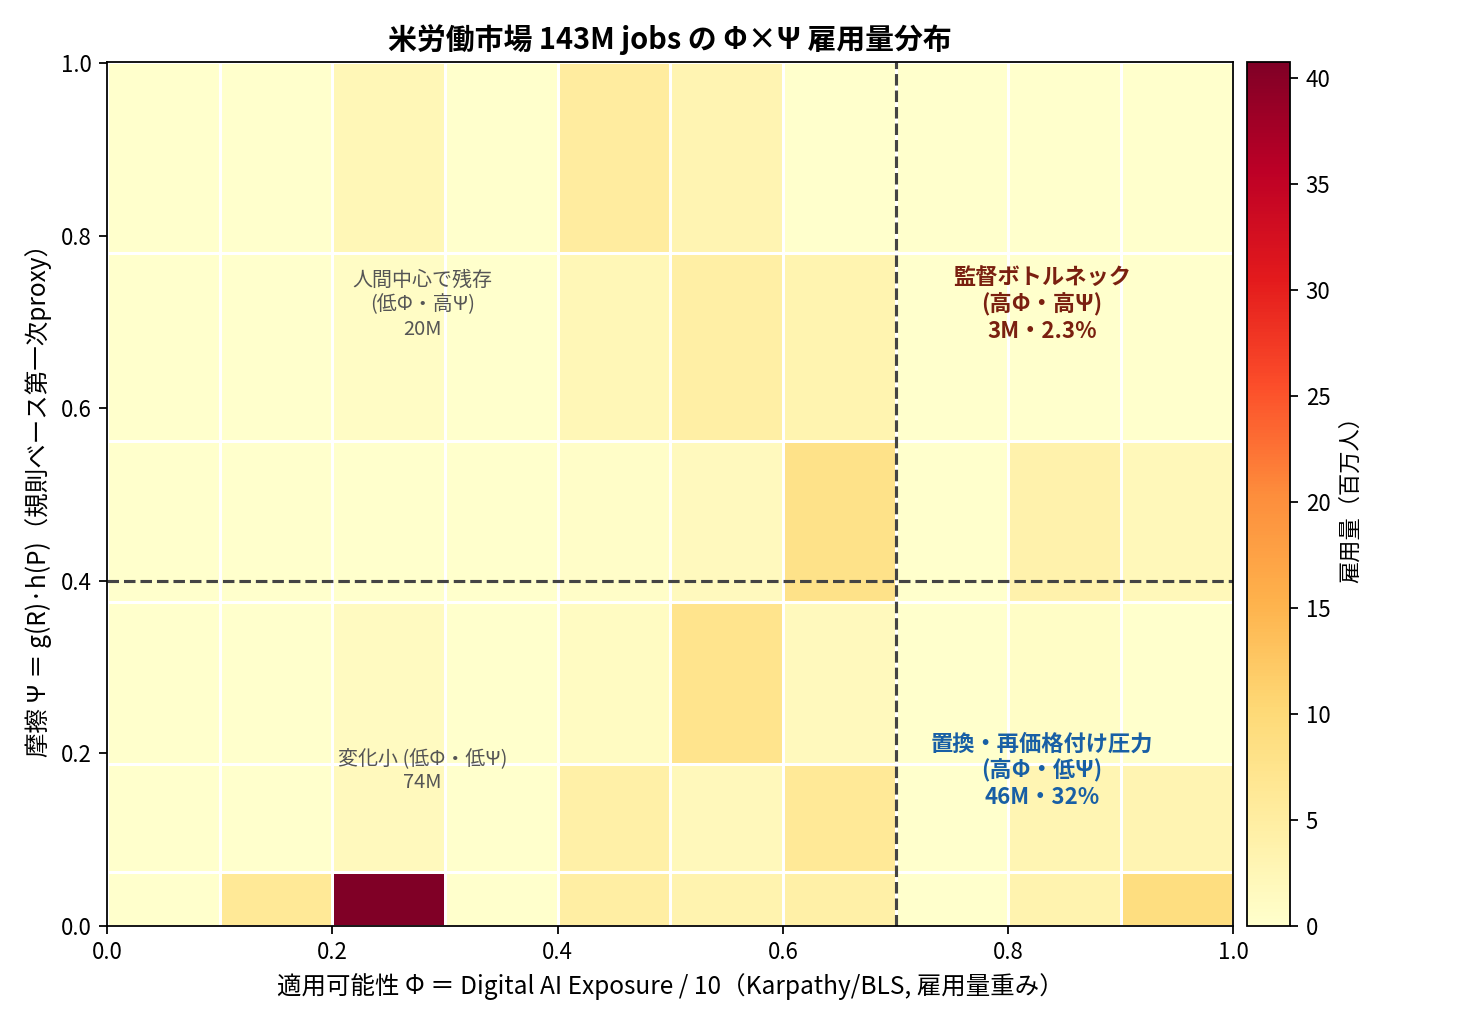
\includegraphics[width=0.92\textwidth]{figures/usheat.png}
\caption{米労働市場 約143M jobs の $\Phi$（Digital AI Exposure $/10$、Karpathy/BLS）× $\Psi$（規則ベース $R,P$）雇用量分布。高 $\Phi$ 雇用（曝露 $\ge7$、約49M）の大半は低 $\Psi$ 側（置換・再価格付け圧力）に分布し、高 $\Phi$・高 $\Psi$ の監督ボトルネック・セルは少数。}\label{fig:usheat}
\end{figure}

観察される探索的パターンは三つである。第一に、米雇用の約34\%（約49M）が高適用可能性（曝露 $\ge7$）である。第二に、その高 $\Phi$ 雇用のうち高摩擦（監督ボトルネック）に分類されるのは、$\Psi$ の閾値定義により\emph{7\%--35\%}（約3M--17M）に留まる。残りの65--93\%（約33--46M）は低摩擦であり、本モデルでは保護的再編ではなく\emph{置換または再価格付け}の圧力下にある。第三に、高 $\Phi$・高 $\Psi$ のセルは特定の規制・専門帯に集中する——教員、会計士・監査人、経営アナリスト、航空管制官など。対照的に、高 $\Phi$ 雇用の上位（秘書・事務、レジ、顧客対応、各種クラーク、ソフトウェア開発）はいずれも低 $R$・低 $P$ であり、摩擦による保護を欠く。

この分解は、曝露ツールの注意書き（「再編であって置換ではない」）を雇用量で定量化し、かつ逆向きのニュアンスを与える。すなわち\emph{「再編されて残る」のは高曝露雇用の少数派であり、多数派にはそれを守る摩擦が存在しない}。監督ボトルネック効果は労働市場全体の支配的帰結ではなく、責任制約と価格硬直が共在する特定セグメントの現象である。

\begin{rmk}[本適用の限界]
(i) $\Phi$ は LLM 採点、$\Psi$ は規則ベース採点であり、いずれも粗い第一次 proxy である。点推定（とくに7\%対35\%の幅）は $\Psi$ の閾値と米国の専門サービス価格硬直性の評価に感応する。頑健なのは定性的順序（監督ボトルネックは少数派の規制・専門帯に集中）である。(ii) $R$・$P$ スコアは米国の制度文脈に依存し、日本（第7節）とは異なる。(iii) 雇用量は2024年 BLS であり、AI普及に伴う将来の再配分は織り込んでいない。
\end{rmk}

\section*{参考文献}
\small
\begin{list}{}{\setlength{\leftmargin}{1.4em}\setlength{\itemindent}{-1.4em}\setlength{\itemsep}{2pt}}
\item Acemoglu, D. (2024). The Simple Macroeconomics of AI. \textit{NBER Working Paper} No.\ 32487.
\item Acemoglu, D. and Restrepo, P. (2018). Artificial Intelligence, Automation, and Work. \textit{NBER Working Paper} No.\ 24196.
\item Acemoglu, D. and Restrepo, P. (2020). Robots and Jobs: Evidence from US Labor Markets. \textit{Journal of Political Economy}, 128(6), 2188--2244.
\item Aghion, P., Antonin, C. and Bunel, S. (2019). Artificial Intelligence, Growth and Employment: The Role of Policy. \textit{Économie et Statistique}, 510--512, 149--164.
\item Agrawal, A., Gans, J. and Goldfarb, A. (2018). \textit{Prediction Machines: The Simple Economics of Artificial Intelligence}. Harvard Business Review Press.
\item Anthropic (2026). \textit{Anthropic Economic Index}, データ公開版 release\_2026\_06\_26（2026年4月・5月）. Hugging Face データセット \texttt{Anthropic/EconomicIndex}, CC-BY 4.0.
\item Agrawal, A., Gans, J. S. and Goldfarb, A. (2019). Artificial Intelligence: The Ambiguous Labor Market Impact of Automating Prediction. \textit{Journal of Economic Perspectives}, 33(2), 31--50.
\item Agrawal, A., Gans, J. and Goldfarb, A. (2022). \textit{Power and Prediction: The Disruptive Economics of Artificial Intelligence}. Harvard Business Review Press.
\item Bainbridge, L. (1983). Ironies of Automation. \textit{Automatica}, 19(6), 775--779.
\item Autor, D. H. (2015). Why Are There Still So Many Jobs? The History and Future of Workplace Automation. \textit{Journal of Economic Perspectives}, 29(3), 3--30.
\item Baumol, W. J. (1967). Macroeconomics of Unbalanced Growth: The Anatomy of Urban Crisis. \textit{American Economic Review}, 57(3), 415--426.
\item Baumol, W. J. (2012). \textit{The Cost Disease: Why Computers Get Cheaper and Health Care Doesn't}. Yale University Press.
\item Brynjolfsson, E., Li, D. and Raymond, L. R. (2025). Generative AI at Work. \textit{Quarterly Journal of Economics}, 140(2), 889--942.
\item Catalini, C., Hui, X. and Wu, J. (2026). Some Simple Economics of AGI. \textit{arXiv:2602.20946}.
\item Dillender, M., Lo Sasso, A. T., Phelan, B. J. and Richards, M. R. (2022). Occupational Licensing and the Healthcare Labor Market. \textit{NBER Working Paper} No.\ 29665.
\item Dillon, E. W., Jaffe, S., Immorlica, N. and Stanton, C. T. (forthcoming). Shifting Work Patterns with Generative AI. \textit{American Economic Review: Insights}.
\item Eloundou, T., Manning, S., Mishkin, P. and Rock, D. (2024). GPTs are GPTs: Labor Market Impact Potential of LLMs. \textit{Science}, 384(6702), 1306--1308. 本稿が用いる職業別曝露スコア（$\alpha,\beta,\zeta$）は、同研究のワーキングペーパー版（arXiv:2303.10130）に付随する公開リポジトリの値による。
\item European Union. Regulation (EU) 2024/1689 laying down harmonised rules on artificial intelligence (AI Act).
\item Felten, E., Raj, M. and Seamans, R. (2023). How will Language Modelers like ChatGPT Affect Occupations and Industries? \textit{arXiv:2303.01157}.
\item Frey, C. B. and Osborne, M. A. (2017). The Future of Employment: How Susceptible Are Jobs to Computerisation? \textit{Technological Forecasting and Social Change}, 114, 254--280.
\item Goldfarb, A., Taska, B. and Teodoridis, F. (2023). Could Machine Learning Be a General Purpose Technology? A Comparison of Emerging Technologies Using Data from Online Job Postings. \textit{Research Policy}, 52(1), 104653.
\item Gao, S., Huang, M. et al.\ (2026). Bounded by Risk, Not Capability: Quantifying AI Occupational Substitution Rates via a Tech-Risk Dual-Factor Model. \textit{arXiv:2604.04464} (v2).
\item Garicano, L. (2025). The Economics of Superabundant AI: Autonomy, Scarcity, and the Future of Work. \textit{NBER Conference Volume on the Economics of Transformative AI}.
\item Graetz, G. and Michaels, G. (2018). Robots at Work. \textit{Review of Economics and Statistics}, 100(5), 753--768.
\item Holmstrom, B. and Milgrom, P. (1987). Aggregation and Linearity in the Provision of Intertemporal Incentives. \textit{Econometrica}, 55(2), 303--328.
\item Humlum, A. and Vestergaard, E. (2025). Still Waters, Rapid Currents: Early Labor Market Transformation under Generative AI. \textit{NBER Working Paper} No.\ 33777（2026年3月改訂。旧題 Large Language Models, Small Labor Market Effects）.
\item Jiang, W., Park, J., Xiao, R. (J.) and Zhang, S. (2025). AI and the Extended Workday: Productivity, Contracting Efficiency, and Distribution of Rents. \textit{NBER Working Paper} No.\ 33536.
\item Karpathy, A. (2025). US Job Market Visualizer. \textit{Open-source research tool}, \texttt{github.com/karpathy/jobs}（BLS Occupational Outlook Handbook 342職業のDigital AI Exposure採点）.
\item McKinsey Global Institute. (2023). \textit{The Economic Potential of Generative AI: The Next Productivity Frontier}.
\item McKinsey \& Company. (2024). \textit{The State of AI in Early 2024: Gen AI Adoption Spikes and Starts to Generate Value}.
\item Noy, S. and Zhang, W. (2023). Experimental Evidence on the Productivity Effects of Generative Artificial Intelligence. \textit{Science}, 381(6654), 187--192.
\item OECD. (2023). \textit{OECD Employment Outlook 2023: Artificial Intelligence and the Labour Market}.
\item Elish, M. C. (2019). Moral Crumple Zones: Cautionary Tales in Human-Robot Interaction. \textit{Engaging Science, Technology, and Society}, 5, 40--60.
\item Parasuraman, R. and Riley, V. (1997). Humans and Automation: Use, Misuse, Disuse, Abuse. \textit{Human Factors}, 39(2), 230--253.
\item Lukac, P. J. et al.\ (2025). Ambient AI Scribes in Clinical Practice: A Randomized Trial. \textit{NEJM AI}. doi:10.1056/AIoa2501000.
\item Peng, S., Kalliamvakou, E., Cihon, P. and Demirer, M. (2023). The Impact of AI on Developer Productivity: Evidence from GitHub Copilot. \textit{arXiv:2302.06590}.
\item Restrepo, P. (2025). We Won't be Missed: Work and Growth in the AGI World. \textit{NBER Conference Volume on the Economics of Transformative AI}.
\item Rotenstein, L. S., Holmgren, A. J., Thombley, R. et al.\ (2026). Changes in Clinician Time Expenditure and Visit Quantity With Adoption of Artificial Intelligence--Powered Scribes: A Multisite Study. \textit{JAMA}, 335(16), 1408--1417.
\item Sinsky, C., Colligan, L., Li, L. et al.\ (2016). Allocation of Physician Time in Ambulatory Practice: A Time and Motion Study in 4 Specialties. \textit{Annals of Internal Medicine}, 165(11), 753--760.
\item Skitka, L. J., Mosier, K. L. and Burdick, M. (1999). Does Automation Bias Decision-Making? \textit{International Journal of Human-Computer Studies}, 51(5), 991--1006.
\item Webb, M. (2020). The Impact of Artificial Intelligence on the Labor Market. \textit{Stanford University Working Paper}.
\item 日本弁護士連合会（各年版）.「弁護士白書」.
\item 日本公認会計士協会（各年版）. 会員数統計および監査関連報告.
\item 日本翻訳連盟（各年版）. 翻訳業界調査報告.
\item 厚生労働省（2024）. 医師の働き方改革に関する検討会 資料.
\item 厚生労働省（各年版）. 医師・歯科医師・薬剤師統計.
\item 矢野経済研究所（各年版）. 語学ビジネス市場に関する調査.
\end{list}
\normalsize
\end{document}
